\documentclass[a4paper,11pt]{article}

%%% ---------------- %%%
%%% --- Packages --- %%%
%%% ---------------- %%%
    \usepackage[utf8]{inputenc}
    \usepackage{authblk}
    \usepackage{graphicx}
    \usepackage[space]{grffile}
    \usepackage{latexsym}
    \usepackage{textcomp}
    \usepackage{longtable}
    \usepackage{tabulary}
    \usepackage{booktabs,array,multirow}
    \usepackage{amsfonts,amsmath,amssymb}
    \usepackage[table]{xcolor}
    \definecolor{lightgray}{gray}{0.9}
    \definecolor{lightergray}{gray}{0.7}
    \usepackage{colortbl}
    
    % macro for arbitray vertical line in tables 
    % see https://tex.stackexchange.com/questions/31441/vertical-line-only-in-one-part-of-a-table
    \def\arrvline{\hfil\kern\arraycolsep\vline\kern-\arraycolsep\hfilneg}
    % -- me 
    \usepackage{lineno}         % for line numbers 
    \usepackage{natbib}         % for citations
    \usepackage[a4paper, left = 2.5cm, right = 2.5cm, top = 2.5cm, bottom = 2.5cm]{geometry}            % page layout
    \usepackage{setspace}       % line spacing
    \usepackage{mathptmx}       % Times new Roman 1
    \usepackage[T1]{fontenc}    % Times new Roman 2
    \usepackage{subcaption}     % subfigure environment
    \usepackage{hyperref}
    \usepackage[labelfont=bf]{caption} % Labels dick gedruckt
    \usepackage[font=small]{caption}  % caption text body small
    \usepackage{microtype}          % to avoid over- or underfull hboxes 
    

    
%%% ---------------- %%%
%%% --- Settings --- %%%
%%% ---------------- %%%
\linenumbers        % line numbers
\doublespacing      % double spaced
\setlength\parindent{0pt}

 % --- Footnotes without marks --- % 
 % see https://tex.stackexchange.com/questions/30720/footnote-without-a-marker
 \newcommand\blfootnote[1]{%
  \begingroup
  \renewcommand\thefootnote{}\footnote{#1}%
  \addtocounter{footnote}{-1}%
  \endgroup
}


% colors 


\title{Should ecologists prefer model- over algorithm-based multivariate methods?}

\author[1]{Jonathan F. Jupke}
\author[1]{Ralf B. Schäfer}
\affil[1]{iES Landau, Institute for Environmental Sciences, University Koblenz-Landau, Fortstraße 7, 76829 Landau, Germany}%

\date{}

\begin{document}

%%% ----------------- %%%
%%% ---Title Page --- %%%
%%% ----------------- %%%

    \maketitle
    corresponding Author: Jonathan F. Jupke, jonathanfrederik@aol.com,
    +49 06341 280-33285\\


    \newpage
    %%% ---------------- %%%
    %%% --- Abstract --- %%%
    %%% ---------------- %%%

        \begin{abstract}%  Less than 250 words 
        %motivation 
            Ecological data sets often record the abundance of several species, together with a set of explanatory variables. 
            %
            Multivariate statistical methods are optimal to analyze such data and are thus frequently used in ecology for exploration, visualization, and inference. 
            %
            Most of the common approaches are algorithmic, they follow mathematical routines like correspondence - or distance-based analyses, which stands in stark contrast to univariate statistics, where data models, assuming specific distributions, are the norm.
            %
            However, through advances in statistical theory and computational power, models for multivariate data have gained traction. 
            %
        %problem statement
            Systematic and simulation-based performance evaluations of these methods are important as guides for practitioners but still lacking.
        %approach
            Here, we compare two model-based methods, multivariate Generalized Linear Models (MvGLM) and Constrained Quadratic Ordination (CQO), with two algorithm-based methods, distance-based redundancy analysis (dbRDA) and Canonical Correspondence Analysis (CCA).
            % 		
            We studied the performance of the methods to discriminate between causal variables and noise variables for 180 simulated data sets covering different sample sizes and data distributions.
        %results
            MvGLM and dbRDA differentiated accurately between causal and noise variables.
            %
            The former had the lowest false positive rate (0.008) while the latter had the lowest false negative rate (0.017).
            %CCA
            CQO and CCA had the highest false negative rate (0.291) and false positive rate (0.256), respectively. 
        %conclusions
           Our study shows that both model- and algorithm-based methods have their place in the ecologists statistical toolbox. 
           % 
        MvGLM and dbRDA are reliable for analyzing species-environment relations, whereas both CQO and CCA exhibited considerable flaws, especially with linear environmental gradients. 
           %
           
        \end{abstract}

    %%% ----------------- %%%
    %%% --- Key-Words --- %%%
    %%% ----------------- %%%

        {\bf Keywords:} 
        %1.
        statistical models,
        %2.
        numerical simulations,
        %3 
        ordination, 
        %4
        multivariate analysis, 
        %5
        variable selection
    \newpage

\newpage

\section{Introduction}

	%------------------------------%
	%&			Erste Absatz:
	%&	Eternal Question + Statisticians point of view 
	%------------------------------%

	Which environmental gradients control species abundances and community composition, is one of the most essential questions in ecology \citep[e.g.][]{Clements1907}  and the current alteration of ecosystems at an unprecedented rate endows it with a new urgency \citep{pacifici2015assessing}. 
	%
	Given the complexity of simulating ecological systems under artificial conditions (e.g. in microcosms), monitoring the abundance or occurrence of taxa across sites with variable  environmental conditions has been one approach to tackle this question.
	%
	Related studies deliver a sites-by-species matrix $\mathbf{Y}$ containing multivariate species abundances, which is then statistically related to  a sites-by-predictor matrix $\mathbf{X}$, containing information on the environmental predictors.
	%
	From a statistical perspective, $\mathbf{Y}$ has many undesirable properties such as
	intercorrelations between variables, 
	e.g. through biotic interactions \citep{morales2015inferring},
	probability distributions other than the normal, 
	more species than sites \citep[\textit{high dimensionality}, especially in DNA barcoding studies, ][]{cristescu2014barcoding},  
	and many zeros, because most species are commonly absent from most sites (\textit{sparsity}) \citep{mcgill2007species}. 
	
	%------------------------------%
	%&		Zweite Absatz:
	%&	Distance Based + Whats wrong with it
	%------------------------------%
    
    While univariate data are routinely analyzed by model-based methods like ANOVA, generalized linear models and linear mixed models, multivariate data are most often analyzed with algorithm-based methods.
    %
    Most of the latter are variations on three basic approaches: i) correspondence analysis, ii) redundancy analysis, or iii) analysis of pairwise distance matrices. 
    %
    Algorithm-based methods have weak links to ecological theory and do not take the data's statistical properties into account. 
    %
    In distance-based algorithms, for example, the researcher implicitly assumes a mean-variance relationship of the data by choosing a certain distance metric. 
	% 
	For instance, Minkowski distances (e.g. Manhattan and Euclidean) assume a constant variance across all mean values \citep{TerBraak1988}
	%
	whereas species abundances often show a quadratic mean-variance relationship \citep{routledge1991taylor, yamamura1999transformation}.
	%
	Whether a distance metric is appropriate depends on the properties of the data and the aim of the study, as each metric extracts different information from the raw data. 
	%
	The choice is complicated by the vast amount of available metrics \citep[see][]{Legendre2012}.
	%
	Misspecification of the relationship by choosing an inappropriate distance metric can lead to erroneous conclusions as demonstrated by \citet{Warton2012}.
	%
	An alternative to algorithm-based analyses that accounts for mean-variance relationships and incorporates ecological assumptions is the model-based approach.\\
 
	%------------------------------%
	%&		Dritte Absatz:
	%&	Model Based Approach
	%------------------------------%

    % -- This is mirrored in the history of CCA and CQO         

	The model-based approach consists of explicitly specifying a statistical model of the process that generated the observed data \citep{Warton2015a}.
	%
	This includes properties such as marginal distributions, overdispersion, zero-inflation, mean-variance relationship, and correlation structure, all of which can be flexibly tailored to the data and the research question.
	%
	While this approach is ubiquitous in univariate analyses \citep[e.g.][]{bolker2008ecological, zuur2010protocol}, it has long been uncommon in multivariate ecological analyses, largely due to the absence of suitable models \citep{anderson2001new}.
	%
    However, advances in statistical theory and computation power have led to a surge of models for multivariate abundance data. 
	%
	Recent examples include Hierarchical Modeling of Species Communities \citep{Ovaskainen2017}, Generalized Joint 
	%
	Attribute Modelling \citep{Clark2017},  and multivariate Generalized Linear Models \citep[MvGLM,][]{Warton2012}.
	
	%------------------------------%
	%&		Vierte Absatz:
	%&			GLMmv
	%------------------------------%
	
	In MvGLM, a separate univariate GLM is fit to each taxon, with each model using the same predictors. 
	%
	Univariate GLMs are a flexible method and are strongly advocated for the analysis of count or occurrence data as they can handle different residual distributions and mean-variance relationships \citep{OHara2010, Warton2011, Szocs2015_b}.
	%
	Extending them to multi-species abundance data was thus a natural starting point for multivariate model-based analyses \citep{Warton2012}.
	%
	The univariate models are combined by summing their test statistics, which allows for inference on the whole community.
	%
	The use of MvGLM, facilitated by an easy-to-use implementation in R  \citep[in the \textit{mvabund} R-package, ][]{Wang2019}, has steadily increased within the ecological community. 
	%
	However, direct comparisons of MvGLM to other methods remain rare, with a few exceptions.
	% 
 	\citet{Warton2012} showed that MvGLMs, in contrast to algorithm-based methods, can differentiate between location (difference in mean) and dispersion (difference in mean-variance relationship) effects. 
 	%
 	%They did not consider variable selection.   
	%
	\citet{Szocs2015} found that MvGLMs performed better or similarly well in terms of statistical power than Principal Response Curves (a form of redundancy analysis) when used for the analysis of ecotoxicological semi-field studies. 
	%
	However, systematic studies of data sets with known properties are lacking and this paucity of studies hampers our capacity to make informed decisions on the selection of methods for multivariate data analysis.\\
	% CQO
% 	Another model-based method based on GLMs is the Constrained Quadratic Ordination (CQO), which is the maximum likelihood solution to Constrained Gaussian Ordination \citep[CGO,][]{Yee2004}, in which species are expected to respond unimodally to latent gradients that are linear combinations of environmental variables \citep{gauch1974ordination}.
% 	%
% 	CQO uses an extension to GLM, the \textit{Vector Generalized Linear Model} \citep[VGLM,][]{yee2003reduced}. 
% 	% CCA
% 	Before growing computation power allowed the exact estimation of CGO, Canonical Correspondence Analysis (CCA) was used as an algorithmic, heuristic approximation. 
% 	%
%     \citet{TerBraak1986} showed that the maximum likelihood estimation of CGO for Poisson-distributed counts can be approximated by correspondence analysis, given that a set of restrictive assumptions hold. 
% 	%
% 	CCA is one of the most widely used and cited multivariate statistical techniques in ecology \citep{Braak2014}.
% 	% db-RDA
% 	Another frequently used technique is Redundancy Analysis, which extends multiple linear regression to multiple response variables. 
% 	%
% 	As it assumes a linear relationship between response and environmental variable it is only appropriate for short gradients.  
% 	%
% 	Distance-based RDA (dbRDA) represents a flexible extension to RDA \citep{Legendre1999, AndersonMati2003}. 
%     %
% 	It calculates an ordination on the distance matrix of the sites-by-species  matrix $\mathbf{Y}$ constrained by the environmental variables $\mathbf{X}$. 
% 	%
% 	dbRDA was highlighted by \citet{Szocs2015}, because the possibility to use asymmetrical distance metrics and avoid the \textit{double-zero problem } \citep{Legendre2012} makes them attractive for sparse data sets. 
% 	%
% 	Generally, comparisons between these different methods are scarce and we are not aware of a study that has compared these different methods to MvGLM. 

	%------------------------------%
	%&		5. Absatz:
	%&		Aim of the Study
	%------------------------------%
	
	We compared the performance of MvGLMs to differentiate between causal and noise variables to three methods of data analysis: 
	%
	Constrained Quadratic Ordination (CQO), which is also model-based, Canonical Correspondence Analysis (CCA) and distance-based Redundancy Analysis (dbRDA), which are algorithm-based.
	%
	We applied the methods to 180 combinations of abundance data sets and explanatory variables.
	%
	The abundance data differed in distributions and sample sizes. 
	%
    Based on the assessment of a variables statistical significance, False Positive Rate (FPR) and False Negative Rates (FNR) were calculated. 
\section{Material and Methods}
    
    %------------------------------%
    %& General approach
    %------------------------------%
    % We generated 180 data sets with varying sample sizes and abundance response shapes. 
    % %
    % Using these data sets, we tested the ability of four multivariate statistical techniques to differentiate between causal and noise variables.  

	%------------------------------%
	%&		Simulations 			
	%------------------------------%

	\subsection{Data Generation}
		Species abundances were simulated as counts, a common abundance measure in ecology \citep{Warton2008}. 
		%
		Abundances were stored in $\mathbf{Y}$, an $N \times S$ matrix of responses, in this case, the abundances of $S$ species, $ s= 1\ ...\ S$, at $N$ sites, $ n = 1\ ...\ N$.
		%
		The species in $\mathbf{Y}$ responded to  environmental variable $x_m$ with one of three different response types: unimodal (\textit{U}), linear (\textit{L}) or bimodal (\textit{B}), as shown in Figure \ref{fig:bivariateExample}.
        %
		These environmental variables are stored in $\mathbf{X}$ an $N \times M$ matrix with $M$ environmental variables, $m = 1\ ... \ M$. 
	    %
	    The simulation process is visualized in Figure \ref{fig:flowchart_simulation}. 
	    
	    
	%--------------------------------%
	%&		Figure: 3d Response shapes	
	%--------------------------------%
		\begin{figure}[ht]
			
			\begin{center}
			    
			    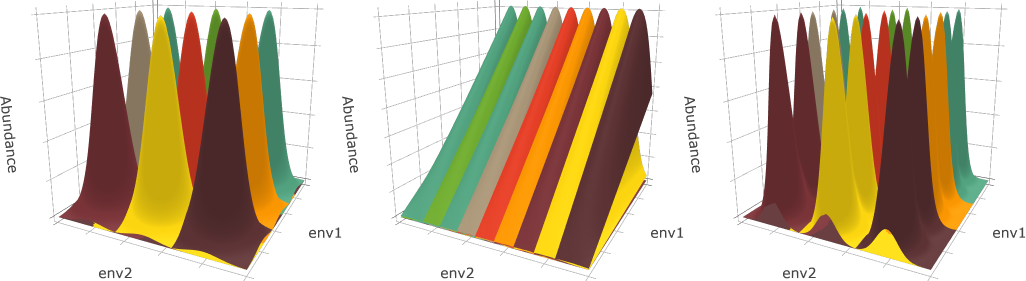
\includegraphics[width = 1\linewidth]{figures/Communities_trimmed_appended.png}     
			   	\caption{
			                Simulated abundance responses along two causal variables (\textit{env1} and \textit{env2}). 
                			%
                            Response combinations are: unimodal-unimodal (left), unimodal-linear (middle) and unimodal-bimodal (right). 
                			%
                			The vertical axis indicates abundance. 
                			%
                			The different colors represent different species.
                			%
                			All the examples show the unsampled abundance matrix
                			$\mathbf{Y_{Large}}$.
			            }
			\label{fig:bivariateExample} 
			\end{center}
			

		\end{figure}
        
		%------------------------------%
		%&		Environmental Gradients				
		%------------------------------%        
        %
		We simulated abundances along two environmental gradients \textit{env1} and \textit{env2}, which henceforth will be referred to as causal variables to differentiate them from the noise variables.  
		%
        Both causal variables consist of the natural numbers from 1 to 100. 
        %
        Each possible combination of the two is a site, i.e. the total number of sites N = 10.000.
		%
		$\mathbf{Y_{Large}}$ holds the simulated abundances for all 10.000 sites.
	    %
	    This data set is larger than most ecological field data sets and fitting models to it would have required considerable computation time.
	    %
	    Therefore, we sampled from $\mathbf{Y_{Large}}$ with six different samples sizes (25, 100, 225, 400, 625, and 900) to obtain $\mathbf{Y_{Sample}}$.
        %
        Depending on the sample size $n$, a set number ($\sqrt{n}$) of sampling locations per causal variable were chosen. 
        %
        These locations always included the variable's minimum and maximum values (i.e. 1 and 100), between those, the locations were equidistantly distributed.
		%
		The abundances of all species at all combinations of sampling locations constitute $\mathbf{Y_{Sample}}$.
		%
		All species show the same response type towards each causal variable, but response types can differ between variables (Figure \ref{fig:bivariateExample}). 
	    %
		This setup allows for six communities each with a different combination of response types, including those with identical response types to both variables (Figure \ref{fig:flowchart_simulation}).  
		%
		The communities are labeled with their abbreviated response types, e.g. \textit{LB} for a community  in which species' abundances respond linearly to the first and bimodally to the second causal variable (Figure \ref{fig:bivariateExample}c). \\
		%------------------------------%
		%&		Responses				
		%------------------------------%
		Unimodal responses were simulated using the Gaussian response model \citep{GauchJr1972} expanded to multiple dimensions (Eqn. \ref{eq:GaussianResponseModel}).
		%
		\begin{equation} \label{eq:GaussianResponseModel}
					y_{s, n} = \prod_{m}^{M_{uni}} c_{s,m} \times exp\bigg(-\frac{(x_{m,n} - u_{s,m})^2}{2t^2_{s,m}}\bigg)		
		\end{equation}
		%	
    	where $u_{s,m}$ is the position of the optimum (i.e. the point with the highest abundance) of species $s$ along the environmental variable $m$, $t_{s, m}$ is the tolerance of species $s$ toward that variable and determines the width of the unimodal curve and $c_{s,m}$ is the maximal abundance of species $s$ on environmental variable $m$. 
		%
		$M_{uni}$ is the number of unimodal environmental variables. 
		%
% 		Note that all environmental variables themselves are actually linear and only the response toward them is variable. 
% 		%
% 		To improve readability though, we will refer to environmental variables in the manner that species respond to them. \\
		%
		Linear responses were simulated by multiplying the environmental variables with a coefficient $\beta$ (Eqn. 2).
		%
		\begin{equation}
		 				y_{s,n} = \prod_{m}^{M_{lin}} x_{m,n} \times \beta_{s,m}
		\end{equation}
		%
		Bimodal responses were simulated by adding two unimodal models with different optima $u_{s,m}$.\\
		%
		This way we obtained $M = 2$ abundance values $y_{m,s,n}$ per species and site. 
		%
		To obtain a single abundance $y_{s,n}$ for each species at each site, we multiplied the abundances of each environmental variables.
		%
		By multiplying instead of adding the abundance values, we ensured that a species is absent from sites where its abundance drops to zero for one of the gradients, i.e. is outside of its niche. 

	%------------------------------%
	%&		Figure: Flowchart 	
	%------------------------------%
		
		\begin{figure}[ht]
			\centering
			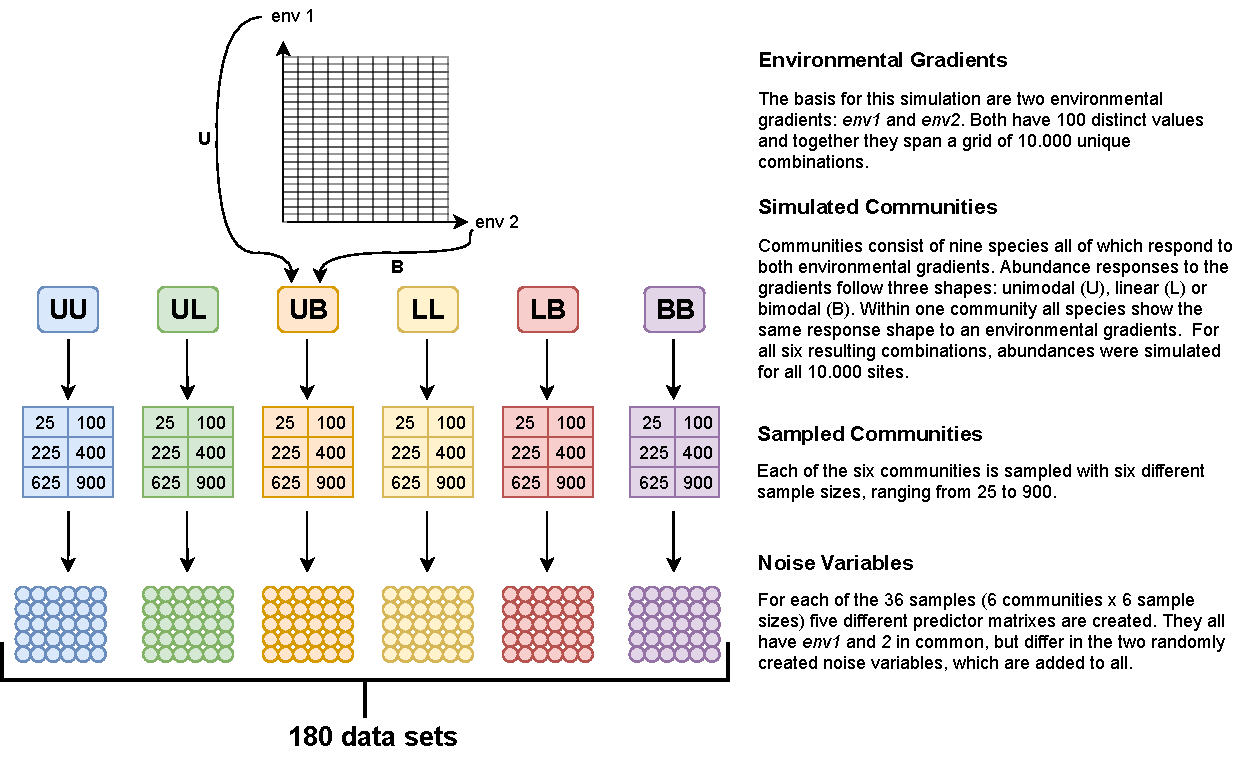
\includegraphics[width=1\linewidth]{figures/190917_MTP_MM_FLOWCHART.pdf}
			\caption{
			        Flowchart of the community simulations. 
			        %
			        The environmental space is comprised out of two variables (\textit{env1} and \textit{env2}) and 10.000 unique sites.
			        %
			        At each site the abundances of nine species are simulated. 
			        %
			        Abundance responses to environmental gradients display three shapes:
			        unimodal (U), linear (L) and bimodal (B). 
			         %
			         All nine species of one community show the same response shape (with varying parameters) to one gradient, but response shapes can differ between gradients. 
			         %
			         All six possible combination of response shapes are sampled with six different sample sizes spanning from 25 to 900.
			        %
                    Before these data are analysed two noise variables are added two $\mathbf{X}$ .
                    %
                    For each response shape - sample size combination, five different pairs of noise variables are appended to $\mathbf{X}$. 
			        }
			\label{fig:flowchart_simulation}
		\end{figure}
	
	%------------------------------%
	%&		Model MISC	
	%------------------------------%
	    
		%
		After the abundances were simulated, noise variables were appended to the model matrix $\mathbf{X}$.
		%
		They were simulated from a standard normal distribution, scaled to the same magnitude as the causal variables and restricted to be orthogonal to them and to each other.  
		%
	    We obtained five different versions of these noise variables by altering the random number generation seed,  giving us five different model matrices per sampled community $\mathbf{Y}_{Sampled}$.  
	    %
	    In total, we sampled six different communities six times each and have five model matrices per sample, resulting in 180 data sets per method of data analysis.\\
		%
        The simulated communities are a simplification of ecological field data. 
        %
        They consist of only nine species and are neither high dimensional nor do they exhibit intercorrelation.
        %
        However, they are not normally distributed and sparse, thereby featuring two of the common issues mentioned above. 
        %
        This relative simplicity eases interpretation of the results.
        %
        Finally, each model was run using five different seeds for random number generation which affects the noise variable. 
        %
        More details on the parameterization of the models are provided in Table SM 1.

    
    \subsection{Overview of Methods}
        
        In the following, the methods of data analysis will be introduced briefly. 
        %
        Each section is concluded with details on how we applied the method in this study.  \\
        %
        \subsubsection{Multivariate Generalized Linear Models}
		A MvGLM consist of $S$ separately fitted univariate GLMs. 
		%
		The likelihood ratio test statistics of all univariate models (i.e. species) are added for each environmental variable to obtain the sum-of-likelihood-ratios statistics.  
		%
		For these statistics, \textit{p}-values related the null hypothesis that a given environmental variable has no effect on the mean community abundance can be calculated. 
		%
% 		Additionally, the relationship between the environmental variable and each species individually can be assessed by their individual likelihood ratio test statistics.   
% 		%
% 		The \textit{p}-values of these are adjusted to multiple testing by controlling the family-wise type I error rate using a resampling-based version of the \textit{Holm's step-down multiple testing procedure} \citep{Westfall1993}. \\
% 		%
% 		%These adjusted \textit{p}-values tend to be very conservative. \\
		%
		We fit MvGLMs with Poisson, negative binomial and Gaussian residual distributions to each community and compared their Dunn-Smyth residual-plots \citep{dunn1996randomized} and Akaike's Information Criteria \citep[AIC, ][]{akaike1974new}.
		%
		The likelihood ratio test statistic was calculated for the best fitting model (least patterns in residuals and lowest AIC).
		%
	    To estimate \textit{p}-values, we used a residual permutation bootstrap with 1000 repetitions \citep{davidsonbootstrap}.
	
	%------------------------------%
	%&  CQO
	%------------------------------%
        \subsubsection{Constrained Quardratic Ordination}
	    Like the MvGLM, the CQO is related to the GLM. 
		%
		It is based on Vector Generalized Linear Models (VGLMs), which are a further generalization of GLMs.
		%
		All GLMs are special instances of VGLMs, just like linear regression is a special instance of a GLM.
		%
		They are not restricted to the exponential family, include multivariate response models, and can explicitly model other response parameters than the mean (e.g. the variance or higher order moments).
        %
        CQO builds on Reduced Rank-VGLMs, in which the $M$ original predictors are reduced to $R$ latent variables $\nu$. 
		%
		This entails the reduction of the hat matrix $\mathbf{H}$, which holds the regression coefficients $\beta$, to a rank $R$ matrix $\mathbf{H_R}$.
		%
		So unlike a MvGLM, CQO reduces the data's dimensionality and in contrast to most ordination techniques (including dbRDA and CCA), the researcher specifies the number of latent variables (i.e. dimensions)  \textit{a priori}.
		%
		$\mathbf{H_R}$ is decomposed into two matrices $\mathbf{H_R}^T = \mathbf{A}\ \mathbf{C}^T$, where $\mathbf{H_R}^T$ denotes the transpose of $\mathbf{H_R}$.  
		%
		The latent variables $\mathbf{\nu}$ are the linear combinations of the constrained coefficients $\mathbf{C}^T$ and the sites-by-predictor matrix $\mathbf{X}$.
		%
		This means that the higher the constrained coefficient of a given predictor is, the more influence it has on the corresponding latent variable.   
		%
		$\mathbf{A}$ holds the regression coefficient of the latent variables.
        %
		CQO extends this model by adding a quadratic term (cf. Eqn. \ref{eq:CQO1}). 
	
		\begin{equation}\label{eq:CQO1} 
		\eta_s = \beta_{(s)1} + \beta_{(s)2} \nu + \beta_{(s)3} \nu^2	
		\end{equation} 
		
		$\beta_1$ is the intercept term and $\eta$ is the linear predictor. 
        It assumes symmetric and unimodal responses to the latent variables.
		 % 
		CQOs were run with Poisson residual distribution and the canonical log-link function.
		%
		The four explanatory variables were scaled and centered before fitting the models.
		%
		The effective nonlinear degrees of freedom were set to 1.5 as suggested by \citet{yee2015vector}.
		%
		Each model was run fifty times and the deviances of each run were compared. 
		%
		If the lowest deviances are too far apart, the solution might be local and the model should be refitted.  
		%
		Here, we fit the model again, until the difference between the lowest and the fifth lowest deviance no longer exceeds 3. 
		% 
		% General Info - absolute values 
        In its current implementation in the VGAM R-package \citep{VGAM19}, CQO does not provide \textit{p}-values \citep[but see][]{yee2010vglms}. 
        %
        To compare its results with the other methods, we calculated pseudo-\textit{p}-values for the CQO (details of the procedures can be found in the 
        %section 2 of the Supplementary Materials).
        Appendix).
        %
        Shortly, to determine the pseudo \textit{p}-value of environmental variable \textit{m}, we permuted the variable 100 times and fit a CQO to each permuted data set. 
        %
        For every model, the absolute values of the constraint coefficient across both latent variables were added for environmental variable \textit{m}, to obtain the test statistic $\sum C_{\nu_{X_{m}}}$. 
        %
        The proportion of test statistics of permuted data sets, that were larger than that of the unpermuted data set, is the pseudo-\textit{p}-value. 
        %
	    All models were fit with rank 1 and 2.
		%
		The optimal number of ranks was found to be 2 for all models, determined by the AIC as proposed by \citet{yee2003reduced}.\\

	%------------------------------%
	%&  CCA
	%------------------------------%
	\subsubsection{Canonical Correspondence Analysis}
	 CCA is the heuristic solution to Restricted Gaussian Regression \citep{Zuur2007}. 
	 %
	 In the latter, one tries to estimate the parameters \textit{u}, \textit{t}, and \textit{c} of a Gaussian response model (see Eqn. \ref{eq:GaussianResponseModel}), but instead of the measured environmental variables, their linear combinations are used as $x$. 
	 %
	 Though it is possible to estimate the parameters with iteratively reweighted least squares in a GLM, this was to computationally intensive at the time the method was proposed by  \citet{GauchJr1972}.
	 %
	 Instead, \citep{TerBraak1986} proposed to approximate the results by CCA, which is valid as long as: all species have equal tolerances $t$ and maximal abundances $c$, their responses are unimodal and symmetrically bell-shaped and their optima $c$ are spread uniformly in the ordination space. 
	 These assumptions are collectively known as the \textit{species packing model}.
	 %
	 \citet{Palmer1993}, \citet{Johnson1999} and \citet{Zuur1999} confirmed the validity of the approximation and its robustness towards violations against the species packing model in simulation studies.
	 %
	 Today, CCA is one of the most widely used and cited multivariate statistical methods in ecology \citep{Braak2014}.\\
		%
		An iterative algorithm is used to obtain estimates. 
		%
		First, arbitrary values are assigned to the site scores (positions of sites in latent variable space, $\mathbf{Z}$). 
		%
		These are used to calculate the species optima $u$ (henceforth species scores) as in Eqn. \ref{eq:CCA_species_scores}.
		%
		\begin{equation}\label{eq:CCA_species_scores}
		\mathbf{u} = \mathbf{D}_c \mathbf{Y}^t \mathbf {Z}
		\end{equation}
		%
		Where $\mathbf{u} = (u_1\ ...\ u_S)^t$, $\mathbf{D}_c$ is a diagonal matrix with the abundance of species $s$ across all sites as its $s,s$-th element and $\mathbf{Y}^t$ denotes the transpose of $\mathbf{Y}$.
		%
		The species scores are in turn used to calculate the site scores as their weighted average $\mathbf{Z}_{wa}$ (Eqn. \ref{eq:CCA_site_scores}) 
		%
		\begin{equation} \label{eq:CCA_site_scores}
			\mathbf{Z}_{wa} = \mathbf{D}_r^{-1} \mathbf{Y} \mathbf {u}
		\end{equation}
		%
		where $\mathbf{D}_r$ is a diagonal matrix with the abundance of all species at site $n$ as its $n,n$-th element and $\mathbf{D}_r^{-1}$ denotes the inverse of $\mathbf{D}_r$. 
		%
		$\mathbf{Z}_{wa}$ is regressed against $\mathbf{X}$ to obtain the weighted regression coefficient $\alpha$. 
		%
		\begin{equation}\label{CCA_canocical_weights}
		\alpha = (\mathbf{X}^t \mathbf{D}_r \mathbf{X})^{-1} \mathbf{X}^t \mathbf{D}_r \mathbf{Z}_{wa}
		\end{equation}
		%
		Lastly, $\mathbf{Z}$ is calculated as the product of $\mathbf{X}$ and $\mathbf{\alpha}$. 
		%
		This procedure is repeated until convergence. \\
	    %
		The distance between sites (scaling 1) or species (scaling 2) in a CCA approximates their two-dimensional $\chi^{2}$-distance, i.e. the Euclidean distance between the expected abundances under the null hypothesis, that abundances do not change along environmental variables, and the actual data.
		%
		Explanatory variables were scaled and centered. 
		%
		Hypothesis tests for environmental variables can be conducted using a pseudo-$F$ statistic with permuted residuals  \citep{Legendre2011} and the null hypotheses that the effect of the variable on the response is equal to zero after accounting for the effect of all other variables. 
	    %
	    Hypothesis tests were conducted with 999 permutations.\\
	
	%------------------------------%
	%& dbRDA
	%------------------------------%
	\subsubsection{distance-based Redundancy Analysis}
	    dbRDA is a variation of the commonly used Redundancy Analysis, proposed by \citet{Legendre1999}.
	    %
        It is not based on one specific distance measure but instead can adopt any chosen measure.
        %
		It is the constrained form of Principal Coordinates Analysis (PCoA) \citep{Legendre1999}, which will be shortly addressed here.
		%
		In PCoA, $\mathbf{Y}$ is transformed into a centered distance matrix $\Delta$.
		%
		The columns of the matrix $\mathbf{PC}$ are the eigenvectors of $\Delta$ scaled to a length that is equal to the square root of their eigenvalues \citep{gower1966some}.
		%
		Each row of PC gives the eponymous \textit{Principal Coordinates} of one observation.
		% 
		In a dbRDA, this matrix $\mathbf{PC}$ is linearly related to the explanatory variables by an RDA.
		%
		The dbRDA preserves the distance metric of $\Delta$, which can be metric, semi- or non-metric.
		%
		dbRDA was highlighted by \citet{Szocs2015}, because the possibility to use asymmetrical distance metrics makes them appealing for sparse data sets. 
		%  	
	    We used the Bray-Curtis distance, which is the reciprocal of the Steinhaus coefficient  \citep{motyka1947zadaniach}, to calculate $\Delta$.
	    %
		Negative eigenvalues were corrected with Lingoes correction \citep{lingoes1971some}.
		%
		As in CQO and CCA, environmental variables were scaled and centered. 
		%
		The significance tests for explanatory variables are calculated using a pseudo-F-Statistic in the same manner as for the CCA.\\
		
	\subsection{Comparison of Methods}
        % How did I evaluate the methods look at results
        The benefit of using simulated rather than field data are twofold:
        %
        i) there is a clear dichotomy between causal and noise variables and 
        ii) we know which variable belongs to which group. 
        %
        This enables us to compare the methods in terms of their classification error rates.
        %
        To this end, we calculated false positive (FPR) and false negative rates (FNR) for each method.
        %
        \begin{align}
           FPR &= FP /(TN + FP) \\        
           FNR &=  FN / (TP + FN)
        \end{align}
        where FP is a False Positive, TN a True Negative, FN a False Negative, and TP a True Positive. 
        %
        A false positive occurs when a noise variable is classified as causal, whereas a false negative when a causal variable is classified as non-causal. 
        %
        True positives and negatives are instances where the variable is labeled correctly. 
        %
        An FPR of 0.5 for example would indicate, that half of all noise variables were classified as causal. 
        %
        Variables with a \textit{p}-value lower than the significance level($\alpha$) were classified as causal whereas all variables with $p > \alpha $  were classified as noise.
        %
        To alleviate the problematic dichotomy of statistical significance \citep{Greenland2016}, we use five different significance levels $\alpha$ (0.01, 0.03, 0.05, 0.07 and 0.1).
		%
		This allows us to evaluate trends in classification strength over different thresholds. 
        

	\subsection{Software}
		All simulations and analyses were done in R 3.4.4 \citep{RCT2018}.
		%
		MvGLM were conducted with mvabund 3.13.1. \citep{Wang2019}, dbRDA and CCA with vegan 2.5-2 \citep{Oksanen2018} and CQO with VGAM 1.0-5 \citep{VGAM19}. 
		%
		R-scripts for the simulations as well as the analyses are available on \href{https://github.com/JonJup/GLMmv-Paper} {GitHub}(https://github.com/JonJup/GLMmv-Paper).
		%
		All calculations were conducted on an Ubuntu 18.04 machine with 64-bit, 8 GB RAM and 1.6 GHz.\\
		%
		All datasets and R scripts generated during and/or analysed during the current study are available from the corresponding author on reasonable request.

% !TeX spellcheck = en_US
\section{Results}
		%------------------------------%
		%& 		References 				
		%------------------------------%  
	
		We report the means and standard deviations of \textit{p}-values of MvGLM, CQO, CCA, and dbRDA for all explanatory variables (Table \ref{table:results1::mean-p}), p-values for different response shapes and sample sizes are given in the Tables S 2 - 5.
		
		%------------------------------%
		%& Table: p-values + standard deviations
		%------------------------------% 

        \begin{table*}[ht]
            \centering
        	\caption{
        	    Mean \textit{p}-values $\pm$ standard deviations of the causal (env1 and env2) and noise variables from multivariate Generalized Linear Models (MvGLM), Constrained Quadratic Ordination (CQO), Canonical Correspondence Analysis (CCA), and distance-based Redundancy Analysis (dbRDA) for all models. 
        	    }
            \begin{tabular}{@{}
            >{\columncolor{white}[0pt][\tabcolsep]}
            cccc
            >{\columncolor{white}[\tabcolsep][0pt]} c
            @{}}
                \rowcolor{lightgray}
                & \textbf{MvGLM} & \textbf{CQO}      &  \textbf{CCA}     & \textbf{dbRDA} \\
                \toprule
                \textit{env1}  & $0.006 \pm 0.0275$   & $0.067 \pm 0.127$ & $0.264 \pm 0.433$ & $0.002 \pm 0.007$ \\
                \textit{env2}  & $0.009 \pm 0.0311$   & $0.090 \pm 0.190$ & $0.264 \pm 0.433$ & $0.003 \pm 0.011$ \\
                Noise          & $0.650 \pm 0.280$    & $0.680 \pm 0.268$ & $0.399 \pm 0.348$ & $0.523 \pm 0.256$ \\
                \bottomrule  
            \end{tabular}
            \label{table:results1::mean-p}	
        \end{table*}


	%------------------------------%
	%& 		GLMmv 					
	%------------------------------%
		%------------------------------%
		%& 			In General 			
		%------------------------------%
        In most MvGLMs, negative binomial residual distribution achieved the lowest AIC and the best fit to model assumptions. 
		%  
		The plot of Dunn-Smyth residuals against the linear predictor of \textit{LL} (Figure S 1) showed arched patterns, which could indicate that the residuals were not independent of the explanatory variables. 
        %
        Nevertheless, We used a negative binomial residual distribution because visual inspection of the QQ-Plots suggested that it resulted in a better fit than Poisson or Gaussian distributions. 

		%------------------------------%
		%& 	 p-values 	
		%------------------------------% 
		MvGLMs' \textit{p}-values for both causal variables and all response type combinations were low (Table  \ref{table:results1::mean-p}).
		%
        The \textit{p}-values of the linear variable in \textit{LB} and \textit{UL} and of the bimodal variable in \textit{UB} were higher at the smallest sample size than at higher ones (Table S 2).  
		%
		Otherwise, the samples size had no effect on the \textit{p}-values of the causal variables, which often were minimal (1 divided by the number of permutations + 1) at small sample sizes.
		%
		The \textit{p}-values for noise variables were higher and varied strongly (Figure \ref{fig:result1::p-valueComparison}).
		%
		They only fell below the nominal significance level of 0.05 in three models. 
		%
		All three models had the response combination \textit{LL} and the low \textit{p}-values occurred at the sample sizes 225, 625, and 900 (Table S 2).
		%
		%------------------------------%
		%& 	 FPR/ FNR  	
		%------------------------------%
		%
		The FPR was the lowest of all methods (0.008 at $\alpha = 0.05$) and always well below the respective significance level (Figure 3). 
		%
		Overall, FPRs and FNRs of MvGLMs were very low (Figure \ref{fig:FPNR}).
		%
        Interestingly the \textit{p}-values of noise variables did not show a monotonic positive relationship with samples size, as we expected. 
        %
        Rather the response seemed unimodal in \textit{UU}, \textit{LL}, and \textit{BB}, slightly negative in \textit{LB} and \textit{UL} and positive for \textit{UB} (Table S 2). \\ 
        
        \begin{figure}[h]
            \centering
            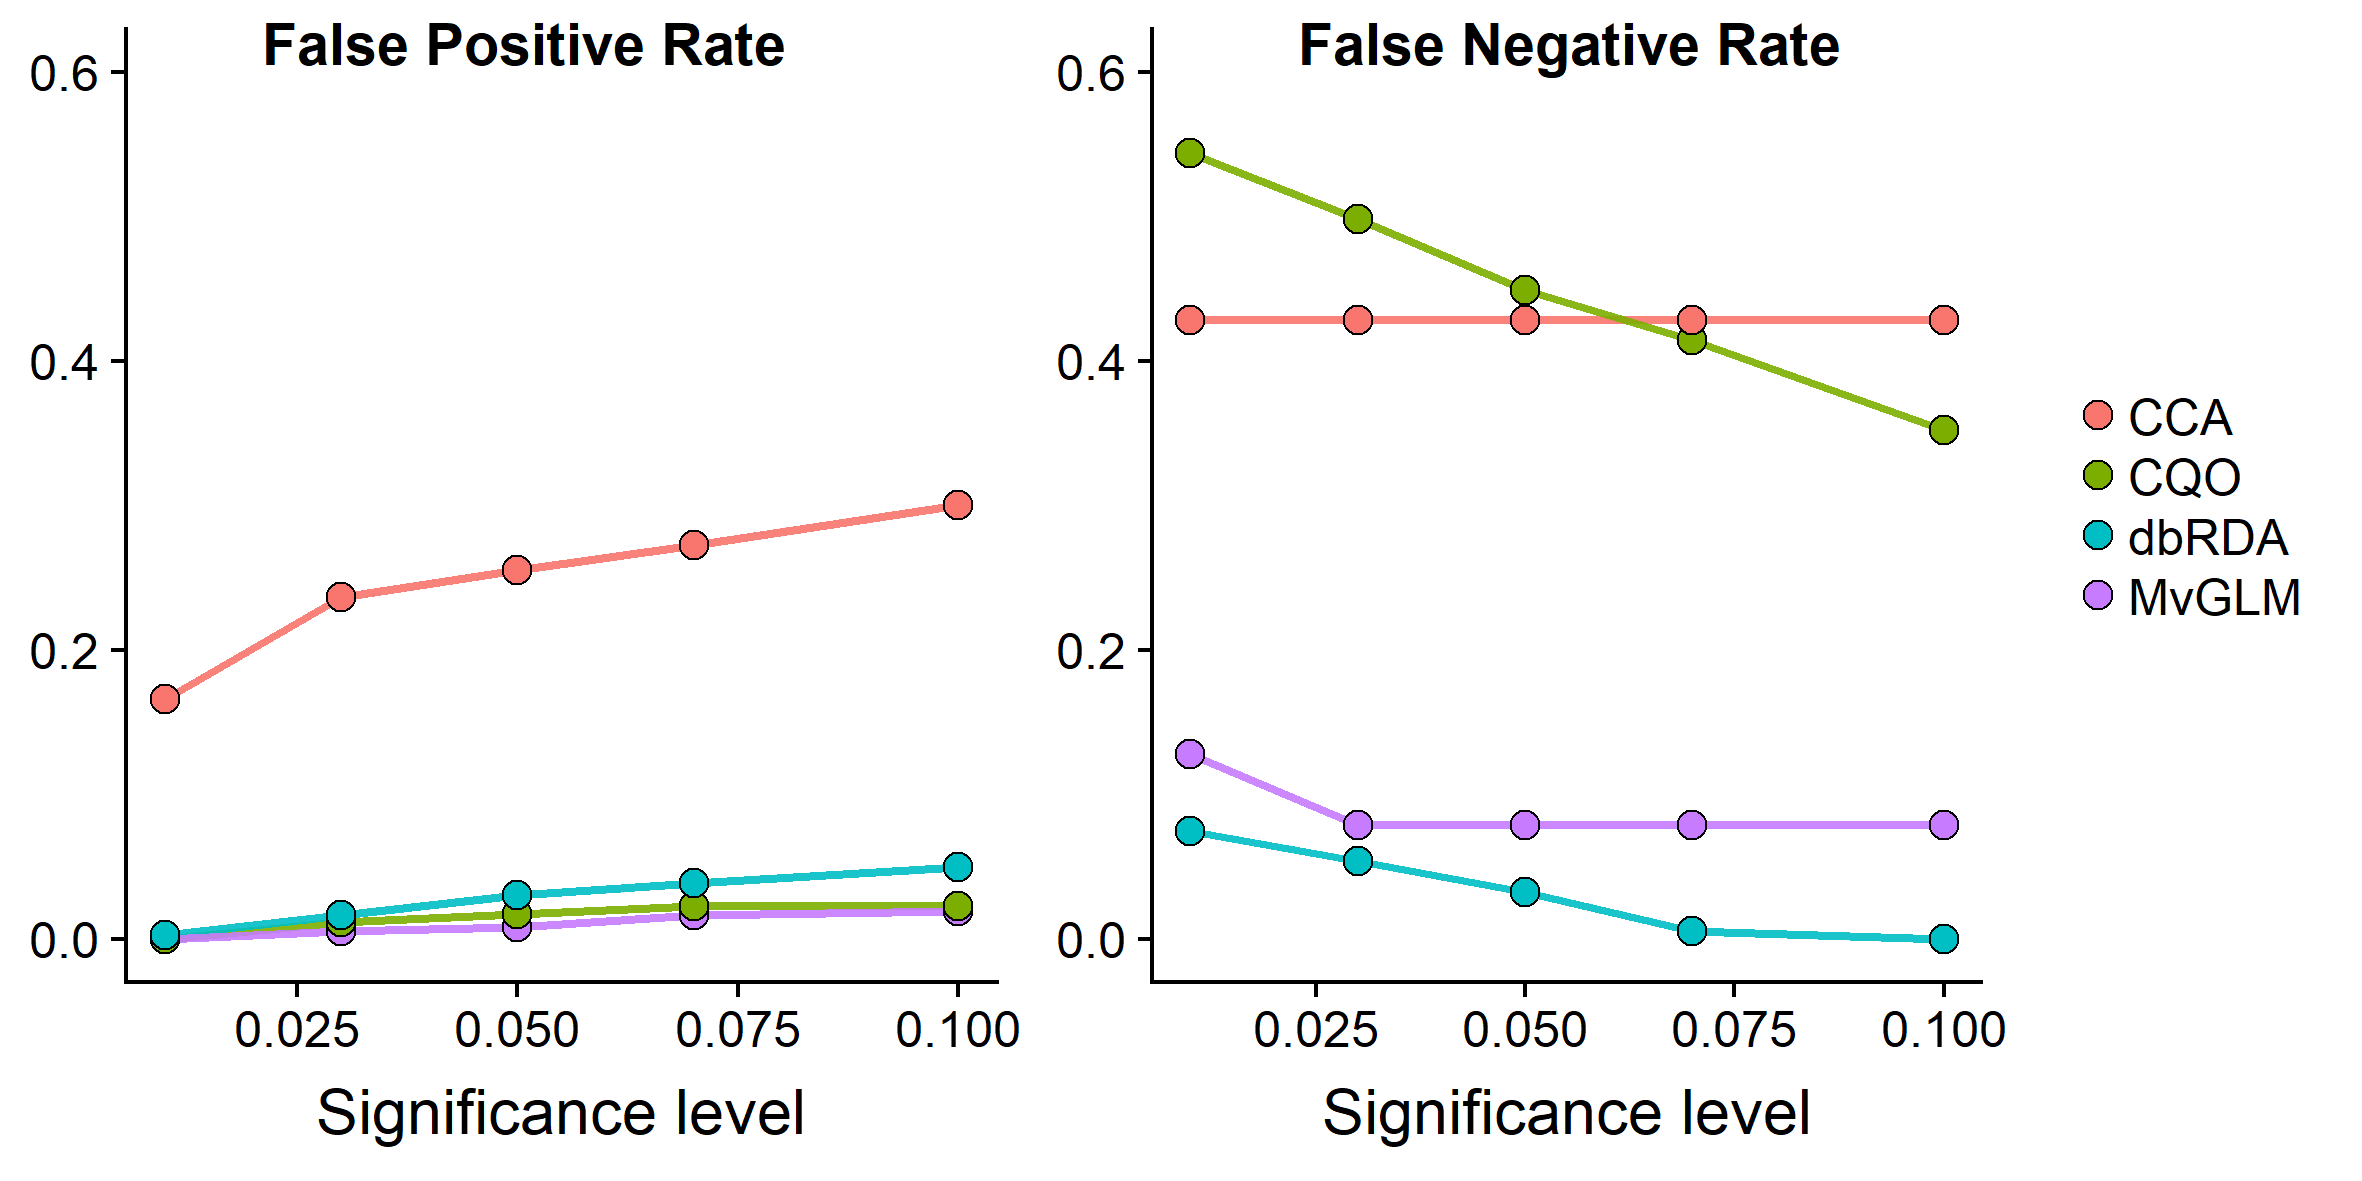
\includegraphics[scale = 0.7]{figures/FPNR.png}
            \caption{False Positive Rate and False Negative Rate of the four statistical methods Canonical Correspondence Analysis (CCA), Constrained Quadratic Ordination (CQO), distance based Redundancy Analysis (db-RDA), and multivariate Generalized Linear Model (MvGLM). }
            \label{fig:FPNR}
        \end{figure}{}
                    
    %------------------------------%
	%& 	CQO			
	%------------------------------% 
	
	CQOs performance strongly depended on the response shape (Figure \ref{fig:result1::p-valueComparison}). 
    %
    It failed to converge for \textit{UB} with sample size 25 and performed best for \textit{UU} and \textit{BB}; both had a FNR of 0 FPRs below the average (0 and 0.06 respectively).
    %
    \textit{UB} performed slightly worse than \textit{UU} and \textit{BB} with an FNR of 0.1 and an FPR of 0.02.
	%
	As was expected, CQO often assigned high \textit{p}-values to linear causal variables (Figure \ref{fig:result1::p-valueComparison}). 
	%
	The mean \textit{p}-value of linear variables was 0.15 and their FNR was 0.53. 
	%
	Both unimodal and bimodal causal variables received higher \textit{p}-values when the other causal variable was linear (Table S 3).
	%
	The mean \textit{p}-value of unimodal variables excluding those from \textit{UL} is $0.006\pm0.022$ compared to $0.036\pm0.084$ for the unimodal variable in \textit{UL}.
	%
	Similarly, the mean \textit{p}-value of bimodal variables except for those form \textit{LB} is $0.004\pm0.015$ and for the bimodal variable in \textit{LB} it is $0.042\pm0.083$.
	%
    This mixed performance leads to relatively high mean \textit{p}-values for the causal variables (Table \ref{table:results1::mean-p}) and accordingly high FNR and FPR (Figure \ref{fig:FPNR}).\\
    
    \begin{figure}
        \centering
        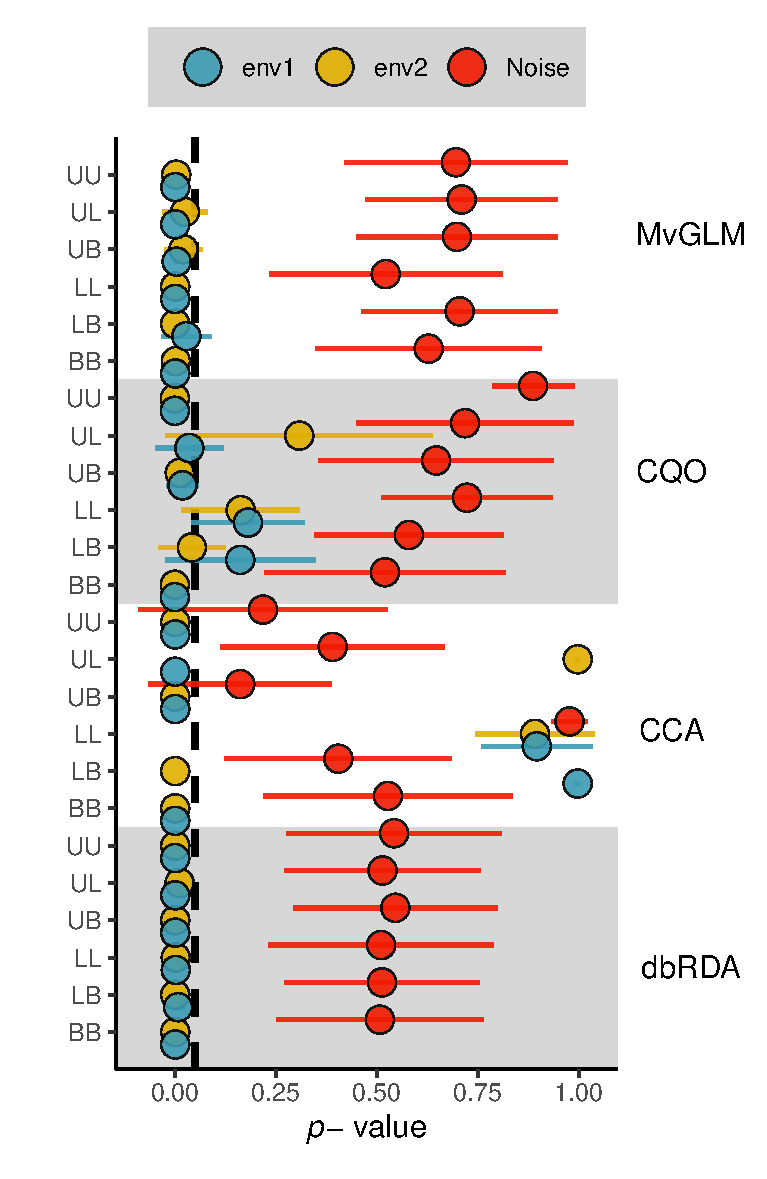
\includegraphics[scale = 0.7]{figures/190912_error_bar.pdf}
        \caption{Mean \textit{p}-values of response combinations (indicated by first letter of response types: unimodal (U), linear (L), bimodal (B)) for multivariate Generalized Linear Models (MvGLM), Constrained Quadratic Ordination (CQO), Canonical Correspondence Analysis (CCA), and distance-based Redundancy Analysis (dbRDA). Blue points are \textit{env1}, yellow points \textit{env2} and red points are noise variables. Bars shows one standard deviation. The vertical, dashed line indicates a \textit{p}-value of 0.05.}
        \label{fig:result1::p-valueComparison}
    \end{figure}
    %------------------------------%
	%& 			CCA					
	%------------------------------% 

		%------------------------------%
		%& 			Variables			
		%------------------------------% 

		CCA has the highest mean \textit{p}-values for causal variables and the lowest for noise ones. 
		%
		Accordingly, the FPR was the highest of all methods (Figure \ref{fig:FPNR}.
		%
		Irrespective of significance level, it is more than one order of magnitude higher than for all other methods.
		%
		These problems are due to two factors: i) high \textit{p}-values for causal linear variables and ii) low \textit{p}-values for noise variables. 
		%
		The mean \textit{p}-value for causal linear variables is $0.963\pm0.094$. 
		%
        Additionally, CCAs of \textit{LL} with sample sizes 400 to 900 produced constrained inertias (explained variance) of 0 and were therefore excluded from significance testing. 
		%
		Noise variable \textit{p}-values were especially low in \textit{UU} and \textit{UB} (Figure \ref{fig:result1::p-valueComparison}), which is interesting since these data sets matched closest with the assumed \textit{species packing model}.  
		%
		In \textit{BB} they were markedly higher (Table S 4). 
		%
        The impact of different sample sizes was negligible in all response combinations (Table S 4).   

	%------------------------------%
	%& 	db-RDA 	
	%------------------------------%

		The dbRDA assigned low \textit{p}-values to most causal variables (Figure \ref{fig:result1::p-valueComparison}).
		%
		The only \textit{p}-values of causal variables above the nominal significance level of 0.05 were those of linear variables at a sample size of 25 (Table S 5).
		%
		However, they were below 0.1, so that the dbRDA had an FNR of 0 at $\alpha = 0.1$.  
		%
		Indeed, the FNR was the lowest of all methods (Figure \ref{fig:FPNR}).
		%
        The \textit{p}-values were relatively similar for all sample sizes (Table S 5). 
		%
        The FPR of dbRDA was relatively high, with 0.031 at $\alpha = 0.05$.  
        %
        The FNR was the lowest of all methods. \\
        %
        Both algorithm-based methods were considerably faster than the model-based ones (Figure S 2).

% !TeX spellcheck = en_US
\section{Discussion}
%------------------------------%
%& 		Repeat what I did		
%------------------------------%
	We analyzed 180 simulated abundance data sets, that differed in response types and sample sizes with four different statistical methods, to assess the methods performance when used to differentiate between causal and noise variables. 
	
%------------------------------%
%& 	one sentence conclusions	
%------------------------------%

    MvGLM and dbRDA performed best showing low FPRs and FNRs for all response combinations and sample sizes. 
	%
    CQO assigned high \textit{p}-values to noise variables resulting in FPRs lower than those of dbRDA but higher than MvGLM's. 
    %
    However, it had the highest FNR for the lower three significance levels, resulting largely from the high \textit{p}-values of linear variables. 
	%
    CCA also assigned high \textit{p}-values to linear variables and additionally assigned low \textit{p}-values to noise variables. 
    %
    The method performed worst in this evaluation, showing the highest FPR at all significance levels and the highest FNR at the two highest significance levels. \\
	
%------------------------------%
%& 			GLMmv				
%------------------------------%
    
    MvGLMs had the lowest FPR of all methods. 
    %
    The three noise variable \textit{p}-values that fell below 0.05 all occurred in \textit{LL} models, which violated the assumption of random residuals and thus would likely be identified as unreliable models.
	%
	The FNR was also low and resulted only through communities with the smallest sample size.
	%
	A drawback of MvGLMs is the long run time due to resampling \citep{Wang2012}.
	%
	The resampling is necessary because it ensures that inferences are valid, even if species are intercorrelated. 
	%
	Resampling observations across independent sites (i.e. rows) accounts for their possible correlation \citep{anderson2001new}. 
    %
	Models that explicitly consider correlation structure avoid resampling and can reduce computation time.
	%
	Such models have been proposed, e.g. by \citet{Jamil2012} who used the site effect of a Generalized Linear Mixed Model to induce equal correlation between all species pairs.
    %
    A clear drawback of this method is, however, that equal correlation between all species is as (im)plausible as no correlation. 
    %
    Structuring the residual covariance matrix is important as the number of parameters that need to be estimated rises quickly (e.g. 55 in the covariance matrix for 10 species).
    %
    MvGLMs can use an unstructured correlation matrix, but this is only advisable for data sets with many more sites than species and is computationally expensive. 
    %
    Another option is shrinking the correlation matrix towards identity using ridge regularization \citep{warton2008penalized, Warton2011a}.
	%
	Both alternatives use Generalized Estimation Equations (GEE) with the sandwich-type-estimator of \citet{Warton2011a}.
	%
	As GEEs do not provide likelihoods, other test statistics than the Likelihood ratio have to be used. 
	%
	Current options are the score and the Wald statistic.
	%
	However, these methods also require resampling, as asymptotic marginal distributions of regression parameters for GEEs are not specified for data sets with more species than sites.
	%
    Testing these methods on data sets with known correlation structures could highlight stronger performance differences, as the other methods lack adjustments to these properties.
    %
	MvGLMs are the only method considered here that does not reduce the dimensions of the data.
	%
	Visualizing the multidimensional data is difficult as no easy-to-use and interpret method for MvGLMs is available. \\

%------------------------------%
%& 		dbRDA		
%------------------------------%
    dbRDA was least influenced by different response types and sample sizes. 
    %
    These properties, together with the low FPR and FNR and the modest computation time make it an excellent method for cultivate analysis in ecology.
	%
	However, the FPR was higher than that of both model-based methods.
	%
	Small \textit{p}-values were scarce for noise variables but occurred at all samples sizes and response types. 
	%  
	dbRDA's good performance is in concert with other simulation studies \citep[e.g.][]{Roberts2009}.
	%
	These results are only valid for the Bray-Curtis distance metric, which was used here.
	%  
	Other measures would likely produce different results, 
	therefore the selection of an appropriate metric is a crucial step in any dbRDA analysis.
	%  
	Having to choose a single metric can be avoided by using consensus RDA \citep{Blanchet2014}.
	% 
	In this method, multiple dbRDAs are run, only differing in their distance metric. 
	%
	Site scores on statistically significant axes are combined into one matrix, which acts as a response matrix in a new RDA. 
	%
	This method extracts the information that is common to all individual dbRDAs.
	%
	Simulation studies comparing properties of consensus RDA with those of individual dbRDA and other methods, algorithm- or model-based, are lacking.
	% 
	Another avenue for the future development of distance-based algorithms, in general, would be novel distance metrics, but their development is pending (M. J.Anderson, pers. comm.).\\

%------------------------------%
%& 				CCA				
%------------------------------%

	The CCA performed worst of the methods tested and assigned high \textit{p}-values to all linear variables.
	%
	As CCA assumes unimodal gradients, which are more frequent than linear ones in nature \citep{Oksanen2002}, this was expected.  
	%
	This study confirmed, that CCA should be avoided if exploratory analyses indicate linear relationships, which can occur if the sampled range of a gradient is short relative to the species' tolerance. 
	%
	Noise \textit{p}-values were lower than in other methods.
	% 
	Most of the low \textit{p}-values for noise variables occurred in communities with uni- or bimodal responses. 
	%
	This is surprising, given that \textit{UU} fits the expectations of the species packing model perfectly and bimodal models deviate only slightly.
	%
	Newer approaches to CCA that can correct for zero inflation \citep{Zhang2012} or non-linear relationships between predictor and response variable \citep{Makarenkov2002} are available but not widely used. 
	%
	Indeed, all of the methods we tested here can include quadratic terms which would most likely have resulted in better fitting models for unimodal and bimodal predictors. 
	%
	Their application is uncommon in CCA and RDA and could be the scope of a future studies.

%------------------------------%
%& 			CQO					
%------------------------------%

	Similar to the CCA, CQO assigned high \textit{p}-values to linear variables. 
	%
    It also assumes unimodal responses and the non-detection of causal linear gradients was expected. 
    %
    The \textit{p}-values for linear variables of CQO were markedly lower than in the CCA, however, the \textit{p-value} of the second variable in these models tends to increase. 
    %
    Overall, this resulted in a high FNR.
	%
	The FPR however, was lower than for both algorithm-based methods but slightly higher than for MvGLM. 
	%
	These results reflect the performance of CQO when combined with our approach to compute \textit{p}-values, which to our knowledge, is novel. 
	%
CQO has only rarely been used in ecological studies and mostly within fisheries research (e.g. \citet{Vilizzi2012}, \citet{Top2016} and \citet{Carosi2017}). 
	% 
	\citet{TerBraak2015} suggest that this is due to limitations on the number of species that can be included, a steep learning curve and numerical instability. 
	%
	This study confirmed that in its current state the method has issues with linear response types but can handle alteration of the symmetrical unimodal bell-shape. \\

% ---------------------------------------- %
%&		Andere Vergleichende Studien		
% ---------------------------------------- %
 
 	Our study is the first to directly compare the methods. 
 	%
 \citet{Warton2012} compared MvGLMs to CCA and RDA (not dbRDA).
 	%
 	They showed that only MvGLMs successfully differentiate between the location effect (difference in means) and dispersion effect (difference in variance). 
 	%
 	Comparative studies of multivariate methods, in general, are common. 
 	%
 	Especially ordination techniques like CCA and RDA were subject to extensive testing in the 1970s and 1980s \citep[e.g.][]{GauchJr.1972, GauchJr1977, Kenkel1986}. 
 	%
 	To our knowledge, \citet{Roberts2008} and \citet{Roberts2009} are the only studies that systematically compared dbRDA to other methods. 
 	%
 	Both compared dbRDA, CCA and Multidimensional Fuzzy Set Ordinations. 
 	%
 	\citet{Roberts2008} used simulated data sets to this end, whereas \citet{Roberts2009} used four different field data sets. 
 	%
 	Both studies concluded that dbRDA outperforms CCA, as it does in this study.
 	%
 	CQO is occasionally tested in comparisons of individual and community level species distribution models (e.g. \citet{Baselga2009} and \citet{Maguire2016}),
 	where they are an instance of the latter.
 	%
 	Generally, they exhibited a similar performance as classical models (e.g. GLMs or Regression Trees). \\

%------------------------------%
%& 		Simulated Data			
%------------------------------% 
    The realism of the simulated communities could be improved by using more complex response patterns like beta-functions \citep{austin1994determining}, which add asymmetries to bell-shaped curves.
	%
	However, in a study of \citet{Oksanen2002} only about 20\% of the responses were strongly skewed, whereas symmetric and bell-shaped responses were most common. 
	%
	Alternatively, asymmetry could be introduced through random terms added to abundances, environmental variables, or both. \citep[e.g.][]{McCune1997}
	%
	When correlated random terms are added to both, this would engender endogeneity (a non-zero covariance between the residuals and one or more explanatory variables). 
	%
	Simulations with induced endogeneity would be interesting as this phenomenon is underappreciated by ecologists \citep{armsworth2009contrasting, fox2015ecological}.
	%
	Observation and measurement are sources of errors in field data sets, and both can be represented in a model via binomial functions as in N-mixture models \citep{royle2004n}.
	%
    This would be interesting to examine the effects of regression dilution \citep{frost2000correcting, McInerny2011}.
 
%------------------------------------------------%
%& Andere Vielversprechende Model-based approaches
%------------------------------------------------%

	Our study shows that model-based multivariate inference can outperform more frequently used algorithm-based methods. 
	%
	The answer to our eponymous question is thus: Not categorically - decisions should be made on a case-by-case basis.
	%
	As model-based methods are still at an early stage, new developments and increases in computation speed can be expected.   
	%
	An especially active area are models using joint probability distributions \citep[e.g.][]{Clark2014, Pollock2014} that estimate the joint distribution of all species conditional on the environmental variables instead of only using the marginal distribution of every species' abundance. 
	%
	A common interest of many joint models is to infer biotic interactions from the residuals of the species-environment interaction, 
	as these two sets of predictors (biotic and abiotic) were shown to have little redundancy \citep{Meier2010}.
	%
	Some of the models also anticipate the growing challenges of Big Data for ecology \citep{Hampton2013}.
	%
	Generalized Linear Latent Variable Models, for example, include latent variables instead of random effects to capture residual correlation, which considerably reduces the size of the variance -- covariance matrix \citep{Warton2015,Niku2017}.  
	%
	In Hierarchical Modeling of Species Communities \citep{Ovaskainen2017} this approach is coupled with a fourth corner model \cite[including species traits, ][]{legendre1997relating} and phylogenetic relationships to create a flexible and comprehensive framework for community data analysis.
	%
	In a similar vein, Generalized Joint Attribute Models allow for different kinds of data (e.g. continuous, discrete counts, ordinal counts, and occurrence) to be included in the same response variable and have outperformed Poisson GLM on discrete count data and a Bernoulli GLM on binary host status data in a recent simulation study \citep{Clark2017}. 
	%
	Lastly, \citet{anderson2019pathway} recently highlighted a combination of the model- and algorithm-based approaches.
    %
    They proposed a copula model of ecological count data \citep[see][for an introduction to copula models]{hofert2018elements}, which consists of i) fitting a copula model to the data, ii) simulating new count data with this copula and iii) visualizing the centroids of the actual data and of the simulated data sets in a PCoA.
    %
    In light of the good performance of dbRDA in our study, this proposal, to join features from both approaches, should be further pursued. 
    %
	It is now essential that ways to infer ecological processes from the modeled patterns develop at a similar pace as these models, to avoid confusing statistical artifacts with genuine biological signals \citep{dormann2018biotic}.
	%
	If this succeeds, a move from algorithm-based towards model-based methods might entail one from the current implicit Gleassonian towards a modern form of Clementsian perspective \citep{Eliot2011}; from asking how do individual species change along environmental gradients towards asking how do communities change as a whole.   
	
\section*{Acknowledgements}
The authors wish to thank Andreas Scharmüller, Stefan Kunz, Sebastian Scheu, Verena Schreiber, and Lucas Streib whose valuable comments  improved the quality of the final document. 
\section*{Author Contributions}
JFJ and RBS conceived the experiment. JFJ conducted the simulation and the analyses. JFJ and RBS wrote the manuscript.
\section*{Data accessibility}
All data as well as scripts are available in the associated Github repository. 
%%% -------------------- %%%
%%% --- Bibliography --- %%%
%%% --------------------- %%%
\bibliographystyle{apalike}
\bibliography{references}
\newpage
\setcounter{figure}{0}
\setcounter{table}{0}

\subsection*{Appendix 1: Calculating pseudo \textit{p}-values for CQO}
 
    Currently, the VGAM R-package \citep[Version 1.1-1,][]{VGAM19} does not implement hypothesis tests regarding the predictors in a CQO. 
    % 
    As we relied on \textit{p}-values to compare the tested methods, we calculated pseudo \textit{p}-values for CQO using a permutation-based test. 
    % 
    We used the absolute sum of constrained coefficients ($ C_{\sum} $) as the test statistic.
    % 
    The constrained coefficient $C_{ij}$ is the weight of the variable $X_i$ on the latent variable $\nu_j$, the higher $C_{ij}$ is the stronger $X_i$ influences $\nu_j$. 
    % 
    By summing $C_{i}$ over all latent variables, we test the impact that $X_i$ has on the model as a whole. 
    % 
    In this summation, we used the absolute values and removed the mathematical sign as these only signify the direction of influence, not its magnitude. 
    % 
    We do not know what distribution to expect from this statistic or if it adheres to a specific distribution. 
    % 
    The method of choice for such cases are permutation-based tests, which produce pseudo \textit{p}-values \citep{legendre2012numerical}. 
    %
    Their general approach is as follows: 
    % 
    A test statistic $T$ is computed for the data set of interest $D$, with $X,Y \in D$. 
    % 
    Some property of $D$ (e.g. the rows of $X$ or $Y$) is permuted $n$-times and the same test statistic is calculated for each of the permuted data sets $D^*$. 
    % 
    The pseudo-\textit{p}-value can then be calculated as: 
    % 
    \begin{center} 
    $p = \displaystyle \dfrac{\sum_{j=1}^n(k_j)}{n + 1}$ \hspace{1cm} 
    with 
    \hspace{1cm} $k_j = \begin{cases} 1 &\text{if\ $T^*_j \ge T$} \\ 0 & \text{else} \end{cases}$\\ 
    \end{center}

    %
    We permuted the predictors. 
    % 
    Each predictor was tested separately so that in any one model only one predictor was permuted while the other remained in their original order. 

\subsection*{Appendix 2: Supplementary figures and tables}   
% \section{Simulation parameters} 
%     Table \ref{tab:SimDet} shows the model parameters used in the simulations. The optimum parameter \textit{u} is the only instance of a parameter that is relevant to both gradients and differs between them. 
% 		%
% 		The different values are separated by forward slashes. 
% 		%
% 		Bimodal gradients require two optima per species. 
% 		%
% 		The used combinations are shown in square brackets. \\
		
		% ------------------------- %
		%& Table: Model parameters 
		% ------------------------- %
		% function from the caption package 
	\captionsetup[table]{name=Table S}
	\begin{table}[!htbp] 
		\centering 
        \caption{
            Model parameters used in simulations. An x indicates that the parameter is not relevant to the respective gradient type. \textit{c} is the maximal abundance, \textit{t} the tolerance, \textit{u} the location of the optimum and $\beta$ the  linear response parameter. Values in square brackets are the pairs of optima for bimodal gradients.
        }
        \label{tab:mvglm:ss} 
        \begin{tabular}{@{\extracolsep{5pt}} cccll}
			\\[-1.8ex]\hline 
            \hline \\[-1.8ex] 
            % Table body 
                %Header 
			    & \textit{c} & \textit{t} & \textit{u} &\ $beta$ \\
			\hline \\[-1.8ex]
				% Row 1 
				\textit{UU} & 100 & 7.5 & 20, 50, 80  & x                 \\
				% Row 2
				\textit{UL} & 100 & 7.5 & 10, 20, 30, 40, 50,60,70,80,90 &  0.1  \\
				% Row 3
				\textit{UB} & 100 & 5   & 20, 50, 80,  [10, 30 ],  [40, 60 ],  [70, 90 ]  & x \\
				% Row 4
				\textit{LL}   & x   & x   & x & 0.1, 0.2125, 0.3250, 0.4375, 0.5500, \\
				&&&& 0.6625, 0.7750, 0.8875, 1.0000 &      \\ 
				% Row 5
			    \textit{LB}  & 100 & 6   & [5, 25], [25, 45], [35, 55], [55, 75], [75, 95] & 0.1   \\
			    % Row 6
				\textit{BB}   & 100 & 6   & [5, 25], [35, 55], [75, 95] & x  \\
			\hline \\[-1.8ex] 
	    \end{tabular}
		\label{tab:SimDet}
	\end{table}
% page break 		
    % function from the caption package 
    \captionsetup[figure]{name=Figure S}
    \begin{figure}[!htbp]
        \centering
        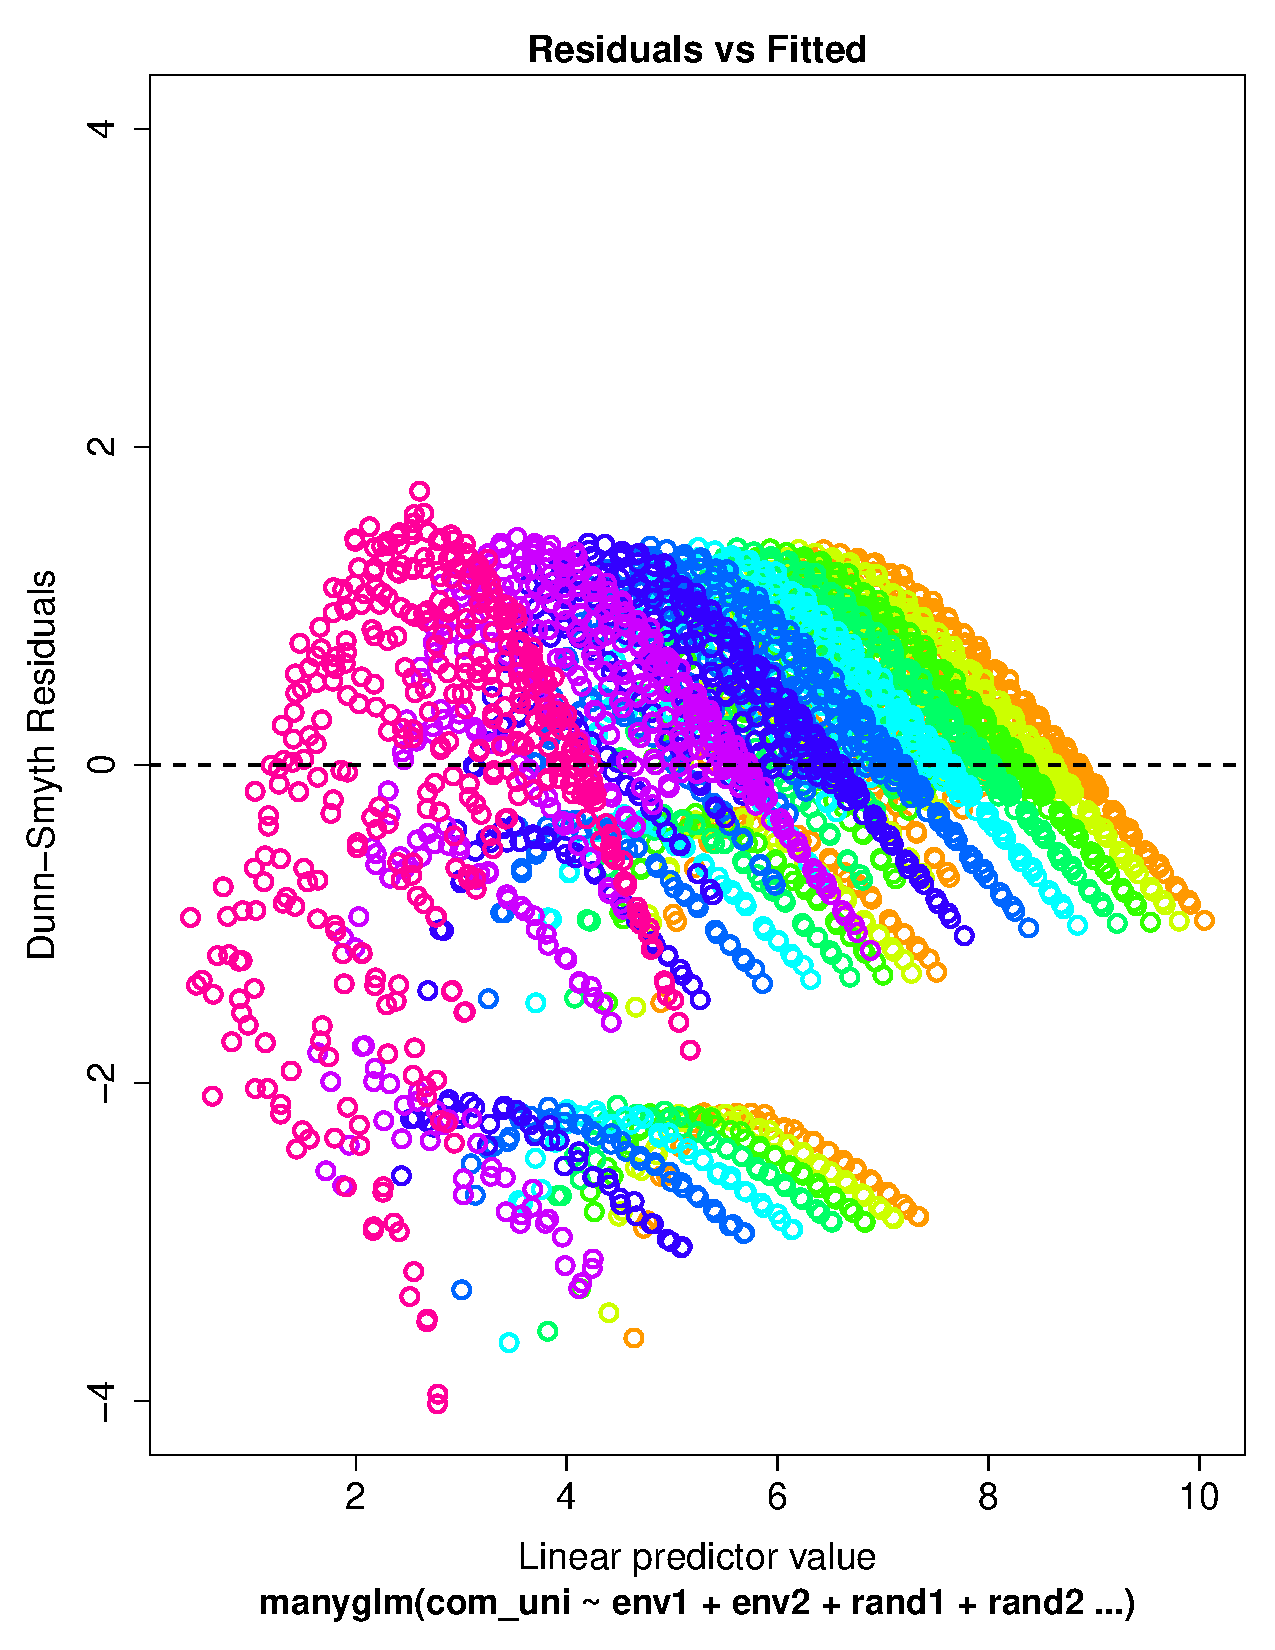
\includegraphics[scale = 0.4]{figures/arched_dunn_smyth.pdf}
        \caption{The Dunn-Smyth residuals of the \textit{LL} community sampled with 400 samples plotted against the linear predictor. A pronounced arched pattern can be observed for each single species (different colors).}
        \label{fig:arched_DS}
    \end{figure}{}
    
  
    
    \begin{figure}[!htbp]
        \centering
        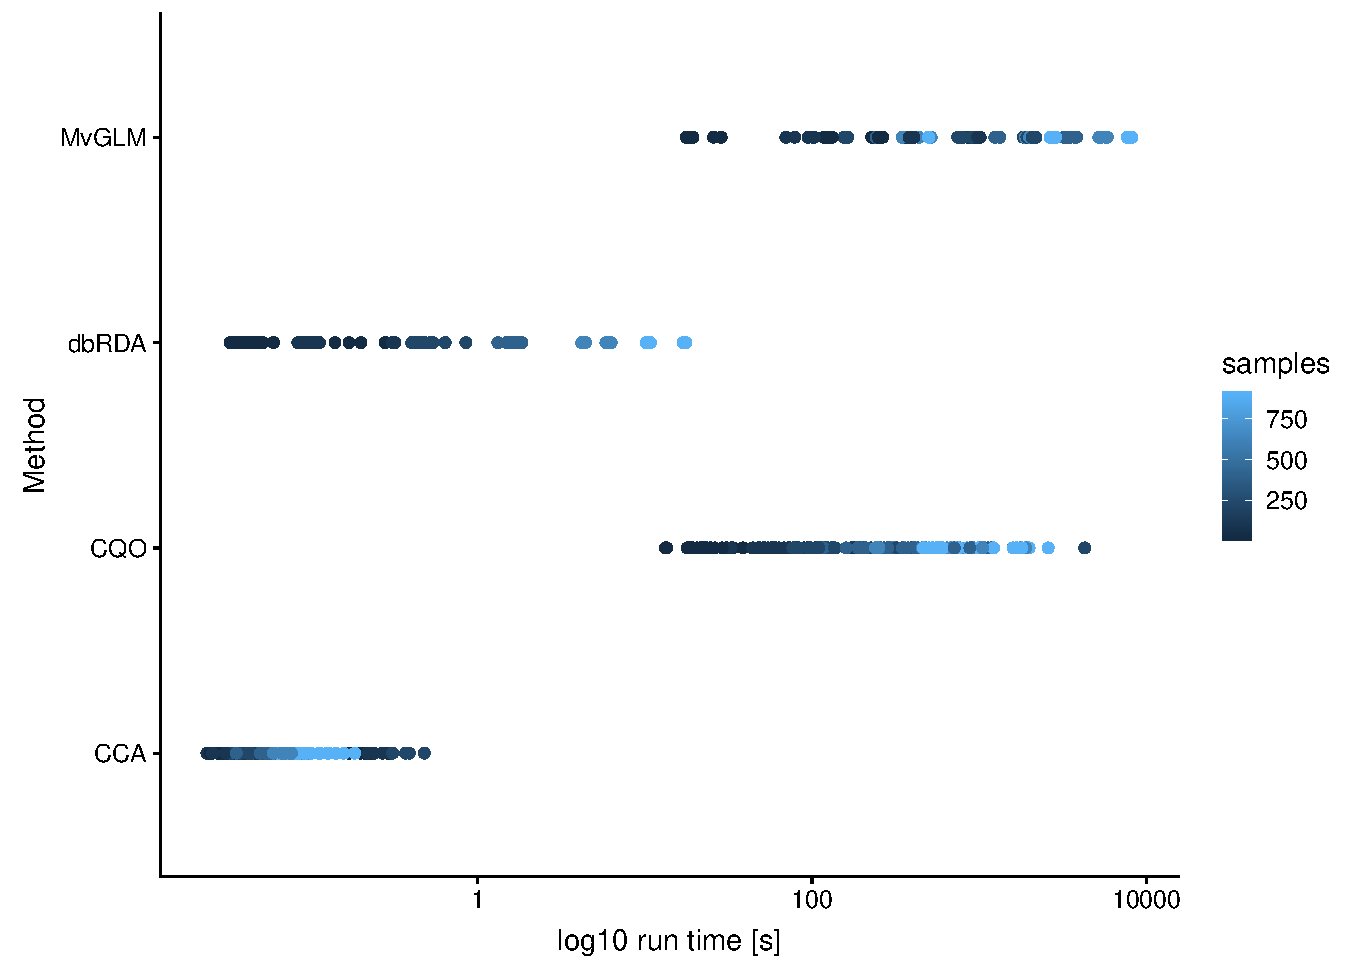
\includegraphics[scale =0.6]{figures/run_timeplot.pdf}
        \caption{Run times of Multivariate Generalized Linear Models (MvGLM), distance-based Redundancy Analysis (dbRDA), Constrained Quadratic Ordination (CQO), and Canonical Correspondence Analysis (CCA). X-axis is scaled with a decimal logarithm. Colors indicate sample sizes.}
        \label{fig:runtime}
    \end{figure}{}

% 	Mean run time of CCA was below one second (s) and that of dbRDA was 4.3 s. 
% 	%
% 	There were no significant differences between different response types or sample sizes. 
% 	%
% 	CQO was the faster model-based method with a mean run time of 365 s.
% 	%
% 	Between response types, speed differed from 175 s (\textit{LL}) to 592 s (\textit{UB}). 
% 	%
% 	Mean run time increased linearly with sample size form 27 s (n = 25) to  972 s (n = 900).
% 	%
% 	MvGLM was the slowest method with a mean run time of 2159 s.
% 	%
% 	Again speed differed between response types and again \textit{LL} was the fastest with  741 s while \textit{BB} was the slowest with a mean run time of 3337 s.
% 	%
% 	Here too, run time increased linearly with samples size form 174 s (n = 25) to 5055 s (n = 900).
% 	%
% 	Note, however, that the times for CQO do not include the calculation of p-values which is quite time-consuming. 
% \section{Further Result Statistics}	

% page break 		
	\newpage	
% 		This section contains all the mean \textit{p}-values at the level of response types or sample sizes.\\
% 		%
% 		Tables \ref{tab:mvglm:ss} and \ref{tab:mvglm:rs} show the mean \textit{p}-values of MvGLMs. 
% 		%
% 		% ------------------------------------------ %
% 		%& TABLE: GLM multivariate p-Value of Classes
% 		% ------------------------------------------- %
\begin{table}[!htbp] 
    \centering 
    \caption{
    Mean \textit{p}-values of Multivariate Generalized Linear Models with standard deviations for combinations of sample size and response type.
    } 
  \label{} 
    \begin{tabular}{@{\extracolsep{5pt}} cccccccc} 
    \\[-1.8ex]\hline 
    \hline \\[-1.8ex] 
    && \multicolumn{2}{c}{env1} & \multicolumn{2}{c}{env2} & \multicolumn{2}{c}{Noise}\\\cmidrule(l){3-4} \cmidrule(l){5-6} \cmidrule(l){7-8}
    %
    && $\mu$ & $\sigma$ & $\mu$ & $\sigma$ & $\mu$ & $\sigma$\\ 
    \hline \\[-1.8ex] 
    UU & $25$ & $0.002$ & $0.001$ & $0.016$ & $0.005$ & $0.342$ & $0.228$ \\ 
    UU & $100$ & $0.001$ & $0$ & $0.001$ & $0$ & $0.612$ & $0.267$ \\ 
    UU & $225$ & $0.001$ & $0$ & $0.001$ & $0$ & $0.697$ & $0.265$ \\ 
    UU & $400$ & $0.001$ & $0$ & $0.001$ & $0$ & $0.849$ & $0.129$ \\ 
    UU & $625$ & $0.001$ & $0$ & $0.001$ & $0$ & $0.875$ & $0.138$ \\ 
    UU & $900$ & $0.001$ & $0$ & $0.001$ & $0$ & $0.801$ & $0.219$ \\ 
    UL & $25$ & $0.001$ & $0$ & $0.146$ & $0.007$ & $0.781$ & $0.162$ \\ 
    UL & $100$ & $0.001$ & $0$ & $0.001$ & $0$ & $0.738$ & $0.210$ \\ 
    UL & $225$ & $0.001$ & $0$ & $0.001$ & $0$ & $0.727$ & $0.283$ \\ 
    UL & $400$ & $0.001$ & $0$ & $0.001$ & $0$ & $0.729$ & $0.258$ \\ 
    UL & $625$ & $0.001$ & $0$ & $0.001$ & $0$ & $0.642$ & $0.250$ \\ 
    UL & $900$ & $0.001$ & $0$ & $0.001$ & $0$ & $0.645$ & $0.272$ \\ 
    UB & $25$ & $0.022$ & $0.003$ & $0.125$ & $0.010$ & $0.477$ & $0.256$ \\ 
    UB & $100$ & $0.001$ & $0$ & $0.001$ & $0$ & $0.596$ & $0.264$ \\ 
    UB & $225$ & $0.001$ & $0$ & $0.001$ & $0$ & $0.737$ & $0.224$ \\ 
    UB & $400$ & $0.001$ & $0$ & $0.001$ & $0$ & $0.788$ & $0.171$ \\ 
    UB & $625$ & $0.001$ & $0$ & $0.001$ & $0$ & $0.784$ & $0.249$ \\ 
    UB & $900$ & $0.001$ & $0$ & $0.001$ & $0$ & $0.811$ & $0.170$ \\ 
    LL & $25$ & $0.001$ & $0.0004$ & $0.001$ & $0$ & $0.406$ & $0.192$ \\ 
    LL & $100$ & $0.001$ & $0$ & $0.001$ & $0$ & $0.587$ & $0.277$ \\ 
    LL & $225$ & $0.001$ & $0$ & $0.001$ & $0$ & $0.514$ & $0.301$ \\ 
    LL & $400$ & $0.001$ & $0$ & $0.001$ & $0$ & $0.574$ & $0.338$ \\ 
    LL & $625$ & $0.001$ & $0$ & $0.001$ & $0$ & $0.593$ & $0.319$ \\ 
    LL & $900$ & $0.001$ & $0$ & $0.001$ & $0$ & $0.460$ & $0.301$ \\ 
    LB & $25$ & $0.166$ & $0.010$ & $0.001$ & $0$ & $0.776$ & $0.162$ \\ 
    LB & $100$ & $0.001$ & $0$ & $0.001$ & $0$ & $0.717$ & $0.222$ \\ 
    LB & $225$ & $0.001$ & $0$ & $0.001$ & $0$ & $0.736$ & $0.285$ \\ 
    LB & $400$ & $0.001$ & $0$ & $0.001$ & $0$ & $0.721$ & $0.257$ \\ 
    LB & $625$ & $0.001$ & $0$ & $0.001$ & $0$ & $0.639$ & $0.269$ \\ 
    LB & $900$ & $0.001$ & $0$ & $0.001$ & $0$ & $0.643$ & $0.275$ \\ 
    BB & $25$ & $0.001$ & $0$ & $0.010$ & $0.002$ & $0.363$ & $0.242$ \\ 
    BB & $100$ & $0.001$ & $0$ & $0.001$ & $0$ & $0.432$ & $0.230$ \\ 
    BB & $225$ & $0.001$ & $0$ & $0.001$ & $0$ & $0.618$ & $0.276$ \\ 
    BB & $400$ & $0.001$ & $0$ & $0.001$ & $0$ & $0.828$ & $0.158$ \\ 
    BB & $625$ & $0.001$ & $0$ & $0.001$ & $0$ & $0.814$ & $0.191$ \\ 
    BB & $900$ & $0.001$ & $0$ & $0.001$ & $0$ & $0.717$ & $0.222$ \\ 
    \hline \\[-1.8ex] 
    \end{tabular} 
    \end{table} 

% page break 		
	\newpage	
	
	 %% -- CQO -- %% 
	 
	\begin{table}[!htbp] \centering 
        \caption{
            Mean \textit{p}-values of Constrained Quadratic Ordination with standard deviations for combinations of sample size and response type.
        } 
        \label{} 
        \begin{tabular}{@{\extracolsep{5pt}} cccccccc} 
            \\[-1.8ex]\hline 
            \hline \\[-1.8ex] 
            && \multicolumn{2}{c}{env1} & \multicolumn{2}{c}{env2} & \multicolumn{2}{c}{Noise}\\\cmidrule(l){3-4} \cmidrule(l){5-6} \cmidrule(l){7-8}
            %
            && $\mu$ & $\sigma$ & $\mu$ & $\sigma$ & $\mu$ & $\sigma$\\ 
            \hline \\[-1.8ex] 
            UU & $25$ & $0$ & $0$ & $0$ & $0$ & $0.820$ & $0.105$ \\ 
            UU & $100$ & $0$ & $0$ & $0$ & $0$ & $0.879$ & $0.082$ \\ 
            UU & $225$ & $0$ & $0$ & $0$ & $0$ & $0.875$ & $0.126$ \\ 
            UU & $400$ & $0$ & $0$ & $0$ & $0$ & $0.917$ & $0.052$ \\ 
            UU & $625$ & $0$ & $0$ & $0$ & $0$ & $0.880$ & $0.134$ \\ 
            UU & $900$ & $0$ & $0$ & $0$ & $0$ & $0.952$ & $0.050$ \\ 
            UL & $25$ & $0.127$ & $0.158$ & $0.289$ & $0.183$ & $0.646$ & $0.146$ \\ 
            UL & $100$ & $0.071$ & $0.098$ & $0.240$ & $0.258$ & $0.612$ & $0.267$ \\ 
            UL & $225$ & $0.004$ & $0.005$ & $0.010$ & $0.012$ & $0.506$ & $0.298$ \\ 
            UL & $400$ & $0.006$ & $0.013$ & $0.087$ & $0.168$ & $0.569$ & $0.196$ \\ 
            UL & $625$ & $0$ & $0$ & $0.519$ & $0.269$ & $0.990$ & $0$ \\ 
            UL & $900$ & $0.008$ & $0.018$ & $0.705$ & $0.401$ & $0.990$ & $0$ \\ 
            UB & $100$ & $0.024$ & $0.023$ & $0.026$ & $0.026$ & $0.654$ & $0.270$ \\ 
            UB & $225$ & $0.026$ & $0.058$ & $0.014$ & $0.031$ & $0.702$ & $0.206$ \\ 
            UB & $400$ & $0.036$ & $0.060$ & $0.002$ & $0.004$ & $0.658$ & $0.274$ \\ 
            UB & $625$ & $0.010$ & $0.022$ & $0.020$ & $0.044$ & $0.583$ & $0.385$ \\ 
            UB & $900$ & $0$ & $0$ & $0$ & $0$ & $0.639$ & $0.337$ \\ 
            LL & $25$ & $0.085$ & $0.048$ & $0.143$ & $0.090$ & $0.400$ & $0.183$ \\ 
            LL & $100$ & $0.154$ & $0.117$ & $0.095$ & $0.062$ & $0.723$ & $0.176$ \\ 
            LL & $225$ & $0.091$ & $0.075$ & $0.081$ & $0.060$ & $0.841$ & $0.102$ \\ 
            LL & $400$ & $0.180$ & $0.137$ & $0.263$ & $0.227$ & $0.761$ & $0.191$ \\ 
            LL & $625$ & $0.281$ & $0.201$ & $0.208$ & $0.191$ & $0.779$ & $0.126$ \\ 
            LL & $900$ & $0.295$ & $0.099$ & $0.188$ & $0.146$ & $0.838$ & $0.116$ \\ 
            LB & $25$ & $0.265$ & $0.127$ & $0.141$ & $0.159$ & $0.619$ & $0.158$ \\ 
            LB & $100$ & $0.097$ & $0.090$ & $0.038$ & $0.058$ & $0.619$ & $0.278$ \\ 
            LB & $225$ & $0.067$ & $0.109$ & $0.006$ & $0.013$ & $0.589$ & $0.272$ \\ 
            LB & $400$ & $0.174$ & $0.237$ & $0.006$ & $0.009$ & $0.586$ & $0.240$ \\ 
            LB & $625$ & $0.204$ & $0.166$ & $0.044$ & $0.061$ & $0.504$ & $0.260$ \\ 
            LB & $900$ & $0.164$ & $0.314$ & $0.020$ & $0.028$ & $0.561$ & $0.218$ \\ 
            BB & $25$ & $0$ & $0$ & $0$ & $0$ & $0.591$ & $0.233$ \\ 
            BB & $100$ & $0$ & $0$ & $0$ & $0$ & $0.359$ & $0.272$ \\ 
            BB & $225$ & $0$ & $0$ & $0$ & $0$ & $0.573$ & $0.299$ \\ 
            BB & $400$ & $0$ & $0$ & $0$ & $0$ & $0.636$ & $0.317$ \\ 
            BB & $625$ & $0$ & $0$ & $0$ & $0$ & $0.421$ & $0.271$ \\ 
            BB & $900$ & $0$ & $0$ & $0$ & $0$ & $0.543$ & $0.353$ \\ 
            \hline \\[-1.8ex] 
        \end{tabular} 
    \end{table}
	
% page break 		
	\newpage		
	
    %% -- CCA -- %% 
    \begin{table}[!htbp] \centering 
        \caption{
            Mean \textit{p}-values of Canonical Correspondence Analysis with standard deviations for combinations of sample size and response type.
        } 
        \label{} 
        \begin{tabular}{@{\extracolsep{5pt}} cccccccc} 
            \\[-1.8ex]\hline 
            \hline \\[-1.8ex] 
            && \multicolumn{2}{c}{env1} & \multicolumn{2}{c}{env2} & \multicolumn{2}{c}{Noise}\\\cmidrule(l){3-4} \cmidrule(l){5-6} \cmidrule(l){7-8}
            %
            && $\mu$ & $\sigma$ & $\mu$ & $\sigma$ & $\mu$ & $\sigma$\\ 
            \hline \\[-1.8ex] 
            UU & $25$ & $0.001$ & $0$ & $0.001$ & $0$ & $0.001$ & $0$ \\ 
            UU & $100$ & $0.001$ & $0$ & $0.001$ & $0$ & $0.467$ & $0.355$ \\ 
            UU & $225$ & $0.001$ & $0$ & $0.001$ & $0$ & $0.093$ & $0.113$ \\ 
            UU & $400$ & $0.001$ & $0$ & $0.001$ & $0$ & $0.349$ & $0.336$ \\ 
            UU & $625$ & $0.001$ & $0$ & $0.001$ & $0$ & $0.153$ & $0.275$ \\ 
            UU & $900$ & $0.001$ & $0$ & $0.001$ & $0$ & $0.247$ & $0.362$ \\ 
            UL & $25$ & $0.001$ & $0$ & $0.987$ & $0.014$ & $0.403$ & $0.288$ \\ 
            UL & $100$ & $0.001$ & $0$ & $1$ & $0$ & $0.329$ & $0.294$ \\ 
            UL & $225$ & $0.001$ & $0$ & $1$ & $0$ & $0.346$ & $0.274$ \\ 
            UL & $400$ & $0.001$ & $0$ & $1$ & $0$ & $0.393$ & $0.317$ \\ 
            UL & $625$ & $0.001$ & $0$ & $1$ & $0$ & $0.436$ & $0.219$ \\ 
            UL & $900$ & $0.001$ & $0$ & $1$ & $0$ & $0.439$ & $0.321$ \\ 
            UB & $25$ & $0.001$ & $0$ & $0.001$ & $0$ & $0.035$ & $0.074$ \\ 
            UB & $100$ & $0.001$ & $0$ & $0.001$ & $0$ & $0.344$ & $0.269$ \\ 
            UB & $225$ & $0.001$ & $0$ & $0.001$ & $0$ & $0.244$ & $0.283$ \\ 
            UB & $400$ & $0.001$ & $0$ & $0.001$ & $0$ & $0.172$ & $0.195$ \\ 
            UB & $625$ & $0.001$ & $0$ & $0.001$ & $0$ & $0.111$ & $0.192$ \\ 
            UB & $900$ & $0.001$ & $0$ & $0.001$ & $0$ & $0.066$ & $0.170$ \\ 
            LL & $25$ & $0.992$ & $0.012$ & $0.997$ & $0.005$ & $0.976$ & $0.031$ \\ 
            LL & $100$ & $0.985$ & $0.009$ & $0.989$ & $0.005$ & $0.994$ & $0.011$ \\ 
            LL & $225$ & $0.712$ & $0.046$ & $0.691$ & $0.031$ & $0.962$ & $0.069$ \\ 
            LB & $25$ & $0.987$ & $0.015$ & $0.001$ & $0$ & $0.398$ & $0.289$ \\ 
            LB & $100$ & $1$ & $0$ & $0.001$ & $0$ & $0.358$ & $0.307$ \\ 
            LB & $225$ & $1$ & $0$ & $0.001$ & $0$ & $0.378$ & $0.278$ \\ 
            LB & $400$ & $1$ & $0$ & $0.001$ & $0$ & $0.412$ & $0.331$ \\ 
            LB & $625$ & $1$ & $0$ & $0.001$ & $0$ & $0.438$ & $0.209$ \\ 
            LB & $900$ & $1$ & $0$ & $0.001$ & $0$ & $0.446$ & $0.321$ \\ 
            BB & $25$ & $0.001$ & $0$ & $0.001$ & $0$ & $0.564$ & $0.286$ \\ 
            BB & $100$ & $0.001$ & $0$ & $0.001$ & $0$ & $0.469$ & $0.341$ \\ 
            BB & $225$ & $0.001$ & $0$ & $0.001$ & $0$ & $0.580$ & $0.301$ \\ 
            BB & $400$ & $0.001$ & $0$ & $0.001$ & $0$ & $0.566$ & $0.314$ \\ 
            BB & $625$ & $0.001$ & $0$ & $0.001$ & $0$ & $0.497$ & $0.343$ \\ 
            BB & $900$ & $0.001$ & $0$ & $0.001$ & $0$ & $0.491$ & $0.330$ \\ 
            \hline \\[-1.8ex] 
        \end{tabular} 
    \end{table}
% page break 		
	\newpage		
	
    %% -- dbRDA -- %% 
    \begin{table}[!htbp] \centering 
        \caption{
            Mean \textit{p}-values of distance-based Redundancy Analysis with standard deviations for combinations of sample size and response type.
        } 
        \label{} 
        \begin{tabular}{@{\extracolsep{5pt}} cccccccc} 
            \\[-1.8ex]\hline 
            \hline \\[-1.8ex] 
            && \multicolumn{2}{c}{env1} & \multicolumn{2}{c}{env2} & \multicolumn{2}{c}{Noise}\\\cmidrule(l){3-4} \cmidrule(l){5-6} \cmidrule(l){7-8}
            %
            && $\mu$ & $\sigma$ & $\mu$ & $\sigma$ & $\mu$ & $\sigma$\\ 
            \hline \\[-1.8ex] 
            UU & $25$ & $0.001$ & $0$ & $0.001$ & $0$ & $0.510$ & $0.302$ \\ 
            UU & $100$ & $0.001$ & $0$ & $0.001$ & $0$ & $0.669$ & $0.304$ \\ 
            UU & $225$ & $0.001$ & $0$ & $0.001$ & $0$ & $0.457$ & $0.238$ \\ 
            UU & $400$ & $0.001$ & $0$ & $0.001$ & $0$ & $0.611$ & $0.275$ \\ 
            UU & $625$ & $0.001$ & $0$ & $0.001$ & $0$ & $0.561$ & $0.173$ \\ 
            UU & $900$ & $0.001$ & $0$ & $0.001$ & $0$ & $0.451$ & $0.275$ \\ 
            UL & $25$ & $0.001$ & $0$ & $0.066$ & $0.010$ & $0.553$ & $0.240$ \\ 
            UL & $100$ & $0.001$ & $0$ & $0.001$ & $0$ & $0.517$ & $0.275$ \\ 
            UL & $225$ & $0.001$ & $0$ & $0.001$ & $0$ & $0.470$ & $0.268$ \\ 
            UL & $400$ & $0.001$ & $0$ & $0.001$ & $0$ & $0.581$ & $0.278$ \\ 
            UL & $625$ & $0.001$ & $0$ & $0.001$ & $0$ & $0.529$ & $0.199$ \\ 
            UL & $900$ & $0.001$ & $0$ & $0.001$ & $0$ & $0.437$ & $0.228$ \\ 
            UB & $25$ & $0.001$ & $0$ & $0.001$ & $0$ & $0.486$ & $0.291$ \\ 
            UB & $100$ & $0.001$ & $0$ & $0.001$ & $0$ & $0.712$ & $0.245$ \\ 
            UB & $225$ & $0.001$ & $0$ & $0.001$ & $0$ & $0.435$ & $0.235$ \\ 
            UB & $400$ & $0.001$ & $0$ & $0.001$ & $0$ & $0.629$ & $0.234$ \\ 
            UB & $625$ & $0.001$ & $0$ & $0.001$ & $0$ & $0.591$ & $0.119$ \\ 
            UB & $900$ & $0.001$ & $0$ & $0.001$ & $0$ & $0.424$ & $0.272$ \\ 
            LL & $25$ & $0.010$ & $0.005$ & $0.009$ & $0.007$ & $0.520$ & $0.219$ \\ 
            LL & $100$ & $0.001$ & $0$ & $0.001$ & $0$ & $0.467$ & $0.261$ \\ 
            LL & $225$ & $0.001$ & $0$ & $0.001$ & $0$ & $0.477$ & $0.261$ \\ 
            LL & $400$ & $0.001$ & $0$ & $0.001$ & $0$ & $0.665$ & $0.293$ \\ 
            LL & $625$ & $0.001$ & $0$ & $0.001$ & $0$ & $0.589$ & $0.290$ \\ 
            LL & $900$ & $0.001$ & $0$ & $0.001$ & $0$ & $0.347$ & $0.298$ \\ 
            LB & $25$ & $0.044$ & $0.008$ & $0.001$ & $0$ & $0.550$ & $0.241$ \\ 
            LB & $100$ & $0.001$ & $0$ & $0.001$ & $0$ & $0.514$ & $0.277$ \\ 
            LB & $225$ & $0.001$ & $0$ & $0.001$ & $0$ & $0.473$ & $0.266$ \\ 
            LB & $400$ & $0.001$ & $0$ & $0.001$ & $0$ & $0.584$ & $0.276$ \\ 
            LB & $625$ & $0.001$ & $0$ & $0.001$ & $0$ & $0.521$ & $0.194$ \\ 
            LB & $900$ & $0.001$ & $0$ & $0.001$ & $0$ & $0.437$ & $0.224$ \\ 
            BB & $25$ & $0.001$ & $0$ & $0.001$ & $0$ & $0.564$ & $0.296$ \\ 
            BB & $100$ & $0.001$ & $0$ & $0.001$ & $0$ & $0.572$ & $0.316$ \\ 
            BB & $225$ & $0.001$ & $0$ & $0.001$ & $0$ & $0.496$ & $0.258$ \\ 
            BB & $400$ & $0.001$ & $0$ & $0.001$ & $0$ & $0.481$ & $0.195$ \\ 
            BB & $625$ & $0.001$ & $0$ & $0.001$ & $0$ & $0.466$ & $0.237$ \\ 
            BB & $900$ & $0.001$ & $0$ & $0.001$ & $0$ & $0.467$ & $0.265$ \\ 
            \hline \\[-1.8ex] 
        \end{tabular} 
    \end{table}
\end{document}
